\documentclass[11pt,a4paper]{article}

\usepackage[utf8]{inputenc}
\usepackage[T1]{fontenc}
\usepackage[english]{babel}
\usepackage{amsmath,amssymb,amsthm}
\usepackage{geometry}
\usepackage{graphicx}
\usepackage{xcolor}
\usepackage{listings}
\usepackage{booktabs}
\usepackage{longtable}
\usepackage{enumitem}
\usepackage{hyperref}
\usepackage[expansion=false]{microtype}

\geometry{margin=2.5cm}
\hypersetup{
    colorlinks=true,
    linkcolor=blue!50!black,
    urlcolor=blue!60!black,
    citecolor=blue!50!black,
}

\definecolor{kw}{rgb}{0.13,0.29,0.53}
\definecolor{str}{rgb}{0.58,0.0,0.0}
\definecolor{com}{rgb}{0.25,0.50,0.35}
\definecolor{bg}{gray}{0.97}

\lstset{
    basicstyle=\ttfamily\footnotesize,
    backgroundcolor=\color{bg},
    keywordstyle=\color{kw}\bfseries,
    stringstyle=\color{str},
    commentstyle=\color{com}\itshape,
    showstringspaces=false,
    breaklines=true,
    frame=single,
    framerule=0.3pt,
    numbers=left,
    numberstyle=\tiny\color{gray},
    language=Python,
}

\newcommand{\code}[1]{\texttt{#1}}
\newcommand{\vect}[1]{\mathbf{#1}}

\title{Hide-and-Seek Drone Swarm \\
       \large CentraleSup\'elec Multi-Agent Systems --- Technical Report}

\date{\today}

\begin{document}

\maketitle

\begin{abstract}
This report describes the design and implementation of a multi-agent
hide-and-seek system in which a single airborne \emph{seeker} drone tries to
spot a group of \emph{hider} drones that hide behind obstacles. The system is
built on top of the CentraleSup\'elec Vol\`iere TP framework: every drone
controller is a Python function that the simulator (\code{standalone\_sim.py})
calls each tick with the current world state, and must return a velocity
command. The contribution lives in the modules around \code{tp\_algos.py}:
(i) an obstacle-consensus law with both an asymptotic linear term and a
barrier term, used by hiders and seeker alike; (ii) a Coulomb-form
inter-agent dispersion consensus on the swarm potential
$V = (k/2)\sum_{i \ne j} 1/\|p_i-p_j\|$ that the hiders descend collectively;
(iii) a forward field-of-view sensor with a single \code{hider\_view\_heading}
function that drives \emph{both} the catch predicate and the rendered cone,
so a hider can never be seen if its on-screen cone does not also see the
seeker; (iv) a shared-memory broadcast channel between hiders; (v) a
\emph{cover-assignment} primitive that solves a deterministic min-cost
matching so each hider takes a distinct cover face relative to the
last-known seeker pose, with a 1\,s / 0.5\,m hysteresis cache that prevents
role-swap chatter; and (vi) a controller-level 3D inter-drone repulsion in
\code{tp\_algos.py} that adds a hard ``never closer than 1\,m'' fence on top
of the per-controller behaviours. The hider mixes a moderate-gain Lissajous
roam (with analytic velocity feed-forward), the obstacle consensus, the
dispersion consensus, the 3D drone fence, and a soft boundary repulsion;
when an alert is fresh the goal target switches to the assigned cover face
and the gain is raised so the hider actually \emph{reaches} the face before
the seeker. The seeker uses the same obstacle consensus plus a stronger
\emph{soft boundary repulsion} of its own (added because the seeker has no
dispersion term pulling it inward), and lands once the referee reports all
hiders caught.
\end{abstract}

\tableofcontents
\clearpage

% ============================================================
\section{Project context and high-level architecture}
% ============================================================

The project is a CentraleSup\'elec TP (2A/3A) on multi-agent systems. The
target hardware platforms are Crazyflie 2 nano-quadrotors (acting as hiders)
and a DJI RoboMaster TT drone (acting as the seeker), flying inside the
school's \emph{Vol\`iere} arena. The pedagogical aim is to use a hide-and-seek
game as an accessible illustration of multi-agent control, both for the
students implementing it and for the children visiting the Vol\`iere.

\paragraph{Rules of the game.}
\begin{itemize}[leftmargin=1.4em]
  \item A single seeker drone (RMTT) cruises the arena on a slow sweep path.
        It \emph{never receives the hiders' positions} -- it has to find them
        with vision.
  \item Several hider drones (CF2) roam the arena. They know the seeker's
        position only through \emph{their own vision} (a forward cone), and
        only communicate sightings to each other through a shared broadcast
        channel.
  \item When the seeker's forward cone contains a hider \emph{and} the line
        of sight is not occluded by an obstacle, the hider is ``caught'' and
        triggered to land.
\end{itemize}

\paragraph{Module decomposition.}
The code base is split into small files that each address one concern:

\begin{longtable}{p{4cm}p{10cm}}
\toprule
\textbf{Module} & \textbf{Role} \\
\midrule
\code{standalone\_sim.py} & The simulator. Owns the world state, calls each
robot's controller in a thread pool, integrates kinematics, detects
collisions, renders the 3D figure. The only edit in this work is the
spawn-list block (4 hiders, 3 obstacles); everything else is upstream. \\
\code{tp\_algos.py} & The required entry-point file (prof requirement). Beyond
the dispatch shims, it hosts a controller-level 3D inter-drone repulsion
(\code{\_compute\_drone\_repulsion\_3d}) and applies it on top of both the
seeker and hider commands. \emph{Edits kept inside the marked
\code{TO BE MODIFIED} blocks.} \\
\code{cf2\_milestone1.py} & Top-level hider controller: composes a goal force
(roam or hide, with analytic Lissajous feed-forward in roam), obstacle
consensus, Coulomb dispersion consensus, and boundary repulsion; switches
modes on the shared seeker-sighting channel. Also exports
\code{hider\_view\_heading}, the single source of truth for the FoV axis
used by both the catch predicate and the rendered cone. \\
\code{cf2\_sensing.py} & The hider's sensing primitives: intent heading and
FoV-cone obstacle sensing on an axis-aligned bounding box (AABB) model. \\
\code{cf2\_consensus.py} & Two consensus laws: the obstacle push (linear +
barrier, used by both hiders and seeker) and the inter-agent dispersion law
(Coulomb-form gradient flow, used by the hiders to maximize pairwise
distances). \\
\code{cf2\_hider.py} & Inter-hider communication (shared seeker-sighting
memory), single-target cover geometry, and the multi-agent cover-assignment
solver (deterministic min-cost matching). \\
\code{rmtt\_seeker.py} & Seeker controller (\code{compute\_seeker\_cmd},
which does \emph{not} accept hider positions) and the \code{can\_see}
predicate shared with the referee and the hiders' seeker-detection logic. \\
\code{game\_referee.py} & Per-frame catch detection using the same
\code{can\_see} predicate as the seeker's vision cone. \\
\code{sim\_viz.py} & Visualization overlays: 3D FoV cones, position trails,
status HUD. \\
\bottomrule
\end{longtable}

\paragraph{Data flow.}
At each tick $t = k\,\Delta t$ ($\Delta t = 0.05\,\text{s}$), the simulator:
\begin{enumerate}[leftmargin=1.4em]
  \item Snapshots all pose arrays so the controllers see a consistent world.
  \item Submits each robot's controller (the public
        \code{tp\_algos.\*\_controller} entry points) to a thread pool. The
        controller returns a target velocity (and for drones, a target
        altitude / takeoff / land flags).
  \item Integrates the returned commands with a simple Euler step, applies
        the actuator-rate saturations, adds a Gaussian position noise term
        ($\sigma = 5\,\text{mm}$ per step).
  \item Calls \code{game\_referee.update\_catches} to mark any catches.
  \item Runs collision detection (boundary, obstacle, robot-to-robot) and
        colours the robots' safety globes red on contact.
  \item Calls \code{sim\_viz.update} to refresh cones, trails and the HUD.
\end{enumerate}

\paragraph{Default scenario.}
The simulator ships with \code{nbRMTT = 1} seeker, \code{nbCF2 = 4} hiders,
and \code{nbObstacle = 3} (Fig.~\ref{fig:arena_overview}):
\begin{itemize}[leftmargin=1.4em,topsep=2pt]
  \item A $1.0 \times 0.5 \times 2.5$\,m pillar at $(-0.5, 1.5, 0)$.
  \item A $0.5 \times 1.1 \times 2.5$\,m pillar at $(0.8, -2.0, 0)$.
  \item A $3.0 \times 1.0 \times 2.5$\,m \emph{central slab} at $(0, 0, 0)$
        which splits the arena into a north room ($y > 0.5$) and a south
        room ($y < -0.5$) and reduces direct sight-lines between them.
\end{itemize}
The two side pillars occupy opposite rooms; together with the slab they
expose, depending on the seeker pose, up to $3 \cdot 4 = 12$ axis-aligned
candidate cover faces -- the four cardinal normals of each box, kept only
when the outward normal points away from the seeker, see
Sec.~\ref{sec:cover}. With four hiders this is overdetermined in most
configurations and the cover-assignment law has slack to spread the swarm
across both rooms. The seeker spawns at $(1.5,\,1.0,\,0)$, just north of
the central slab and just east of the small north pillar; this is its
worst-case spawn because the slab puts the south-room hiders out of
line-of-sight immediately. The four CF2 hiders start at the corners of an
inset rectangle, $(\pm 1.8, \pm 3.8, 0)$. The corner layout satisfies four
simultaneous constraints at $t = 0$: pairwise hider spacing $\ge 3.6$\,m
(well above the 1\,m hard floor of Sec.~\ref{sec:tp-shim}), seeker-to-hider
distance $\ge 2.82$\,m (outside the seeker's $2.0$\,m vision range, so no
hider is in the seeker's cone at spawn -- and the seeker takes off in
state 1 for $3$\,s before catch detection is even active), wall clearance
$\ge 0.7$\,m (outside the 0.6\,m boundary repulsion margin), and obstacle
clearance $\ge 1.05$\,m from every box (well above
$r_\mathrm{safe} = 0.6$\,m). Each
room of the arena starts with two hiders, so the cover-assignment law
always has candidates on both sides regardless of where the seeker's sweep
takes it first.

\begin{figure}[htbp]
  \centering
  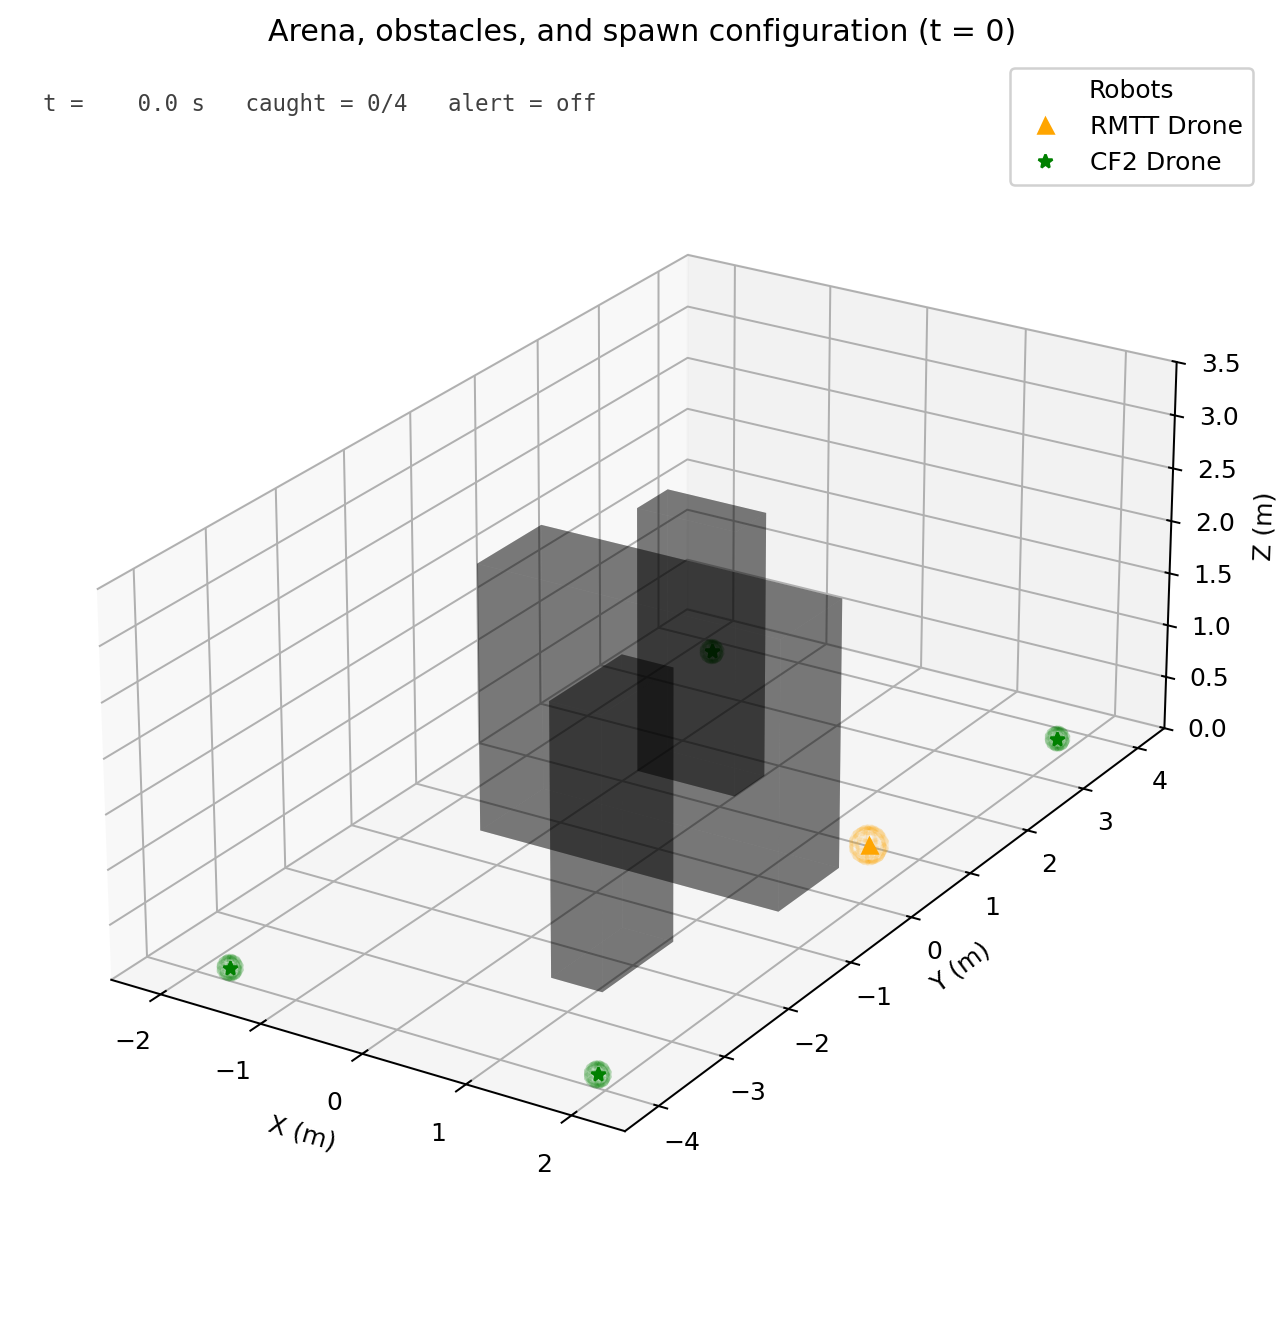
\includegraphics[width=0.85\linewidth]{figures/fig_arena_overview.png}
  \caption{Default scenario at $t = 0$. Seeker (orange triangle) at
  $(1.5, 1.0, 0)$; four hiders (green stars) at $(\pm 1.8, \pm 3.8, 0)$;
  three AABB obstacles in dark grey. The central slab is the dominant
  occluder along the $y$ axis and is what makes the south-room hiders
  invisible to the seeker at spawn.}
  \label{fig:arena_overview}
\end{figure}

% ============================================================
\section{Mathematical model}
% ============================================================

\subsection{State and kinematics}

Each drone is modelled as a point mass with state
$\vect{p}_i = (x_i, y_i, z_i)^\top \in \mathbb{R}^3$ and a velocity command
$\vect{u}_i = (v_x, v_y, v_z)^\top$. The integration is a forward Euler step
with Gaussian noise:
\[
    \vect{p}_i(t+\Delta t) \;=\; \vect{p}_i(t) + \vect{u}_i \Delta t + \vect{\eta}_i,
    \qquad
    \vect{\eta}_i \sim \mathcal{N}\!\left(\vect{0}, \sigma^2 \vect{I}_3\right),
    \qquad \sigma = 0.005\,\text{m}.
\]
Before integration the simulator applies a 3D magnitude clamp at the actuator
limit (\code{clamp\_vel3d} in \code{standalone\_sim.py}).

For CF2 the controller actually returns $(v_x, v_y, z_\mathrm{dist})$ where
$z_\mathrm{dist}$ is the \emph{desired altitude}. The simulator converts it to
a vertical velocity $v_z = z_\mathrm{dist} - z$ and applies the 3D clamp on
$(v_x, v_y, v_z)$ together.

\subsection{Obstacles}

Obstacles are axis-aligned bounding boxes (AABBs) standing on the floor:
\[
    \mathcal{B}_j \;=\; [o_x - \tfrac{s_x}{2},\, o_x + \tfrac{s_x}{2}]
                       \times[o_y - \tfrac{s_y}{2},\, o_y + \tfrac{s_y}{2}]
                       \times[0,\, s_z].
\]
The closest point on $\mathcal{B}_j$ to a query point $\vect{p}$ is the per-axis
clamp of $\vect{p}$ into the box, which collapses to $\vect{p}$ itself when
$\vect{p} \in \mathcal{B}_j$.

% ============================================================
\section{Hider controller (\code{cf2\_milestone1.py})}
% ============================================================

\subsection{Force composition}

The controller assembles four terms:
\[
    \vect{F}_\mathrm{total}
    \;=\; \vect{F}_\mathrm{goal}
        + \vect{F}_\mathrm{obs}
        + \vect{F}_\mathrm{disp}
        + \vect{F}_\mathrm{bnd},
\]
and outputs the planar component of $\vect{F}_\mathrm{total}$ after a
magnitude saturation at $v_\mathrm{max} = 0.55\,\text{m/s}$ (just below the
hardware cap $\text{MAX\_V\_CF2} = 0.6\,\text{m/s}$). The vertical channel
is governed separately: the controller returns a desired altitude
$z_\mathrm{dist}$ that the simulator converts to $v_z = z_\mathrm{dist} - z$
and then clamps with $(v_x, v_y, v_z)$ \emph{together} at
$\text{MAX\_V\_CF2}$. To stop a large $v_z$ from eating the xy avoidance
budget inside that 3D clamp, the controller applies a per-call rate limit
\code{\_Z\_RATE\_LIMIT = 0.01}\,m on $|z_\mathrm{dist} - z|$ before
returning. The result: the xy channel keeps its full $0.55$\,m/s magnitude
even during a vertical excursion, the obstacle barrier of
Sec.~\ref{sec:consensus} stays fully effective, and the drone climbs or
descends at most $0.2$\,m/s.

\subsubsection*{Goal attraction (mode-dependent)}
The goal target is the Lissajous waypoint $\vect{p}_\mathrm{lis}$ in roam
mode and the assigned cover face $\vect{c}_i$ in hide mode
(Sec.~\ref{sec:cover}). The two modes use \emph{different} gain laws:
\[
    \vect{F}_\mathrm{goal}^\mathrm{roam}
    \;=\; k_g^\mathrm{roam}\,(\vect{p}_\mathrm{lis} - \vect{p})
       + \dot{\vect{p}}_\mathrm{lis},
    \qquad k_g^\mathrm{roam} = 0.45,
\]
\[
    \vect{F}_\mathrm{goal}^\mathrm{hide}
    \;=\; k_g^\mathrm{hide}\,(\vect{c}_i - \vect{p}),
    \qquad k_g^\mathrm{hide} = 0.9.
\]
The analytic velocity feed-forward $\dot{\vect{p}}_\mathrm{lis}$ is the
exact time derivative of the Lissajous waypoint, returned by
\code{\_lissajous\_velocity} in \code{cf2\_milestone1.py:83-89}. With the
feed-forward in place, $k_g^\mathrm{roam}$ only has to correct
\emph{tracking error}, not produce the entire chase velocity; this lets it
stay moderate, so a small obstacle excursion or a dispersion push easily
deflects the drone off-path. The cover target is stationary
($\dot{\vect{c}}_i = 0$), so the feed-forward is dropped. The hide gain is
the highest in the controller because the drone must \emph{actually reach}
the assigned face inside the seeker-memory TTL: at $0.9 \times 0.6\,\text{m}
\approx v_\mathrm{max}$ the planar saturation engages whenever the hider
is more than $\sim 0.6$\,m from cover, so the hide command is essentially
``go full speed straight to the face''.

\subsubsection*{Obstacle consensus}
Each sensed obstacle $j$ contributes (see Sec.~\ref{sec:consensus})
\[
    \vect{F}^{(j)}_\mathrm{obs} \;=\;
    \underbrace{k_\mathrm{obs}\,\max(0, r_\mathrm{safe} - d_j)}_{\text{linear}}
    \,\vect{n}_j
    \;+\;
    \underbrace{k_\mathrm{bar}\!\left(\frac{r_\mathrm{safe}}{\max(d_j,\varepsilon)} - 1\right)}_{\text{barrier}}
    \,\vect{n}_j,
\]
with $d_j$ the distance to the obstacle surface, $\vect{n}_j$ the outward
normal (surface $\to$ drone), and $\varepsilon = 0.02\,r_\mathrm{safe}$.

\subsubsection*{Inter-agent dispersion consensus}
\label{sec:disp-force}
Per-agent gradient of the swarm potential
$V_\mathrm{disp}(\vect{p}_1,\dots,\vect{p}_N) = \tfrac{k_\mathrm{disp}}{2}
\sum_{i \ne j} 1/\|\vect{p}_i - \vect{p}_j\|$ in the $xy$ plane:
\[
    \vect{F}^{(i)}_\mathrm{disp}
    \;=\; -\nabla_{\vect{p}_i} V_\mathrm{disp}
    \;=\; k_\mathrm{disp} \sum_{j \ne i}
          \frac{\vect{p}_i - \vect{p}_j}{\|\vect{p}_i - \vect{p}_j\|^{3}},
    \qquad k_\mathrm{disp} = 0.4.
\]
This is a true multi-agent consensus law on the aggregate cost $V_\mathrm{disp}$:
every hider's local law decreases the \emph{same} scalar function along the
joint gradient flow, so the swarm collectively minimizes $V_\mathrm{disp}$,
equivalently maximizes inverse pairwise distances, equivalently spreads as
far apart as the boundary and obstacle constraints allow. Unlike a
short-range repulsion, the law acts at \emph{all} distances -- every hider
always knows about every other hider's pull. Symmetry implies the centroid
of the swarm is invariant under $\vect{F}_\mathrm{disp}$ alone (the goal,
obstacle, and boundary terms then steer the centroid). A numerical floor
$\varepsilon_\mathrm{disp} = 0.05\,\text{m}$ on the denominator avoids a
blow-up if two hiders briefly co-locate. A stricter 3D ``never closer than
1\,m'' separation between \emph{all} flying drones (hiders \emph{and} seeker)
is added on top in \code{tp\_algos.py} (Sec.~\ref{sec:tp-shim}).

\subsubsection*{Boundary repulsion}
Each wall at distance $d$ inside a margin $m = 0.6\,\text{m}$ pushes inward:
\[
    F_\mathrm{bnd}^{(w)} \;=\;
    g_\mathrm{bnd}\!\left(\frac{1}{\max(d,10^{-4})} - \frac{1}{m}\right),
    \qquad g_\mathrm{bnd} = 0.09.
\]
The gain is intentionally small ($0.09$) -- the goal is a gentle nudge, not a
hard bounce.

\subsection{Lissajous roaming path}
\label{sec:lissajous}

Each hider $i$ tracks a 3D Lissajous waypoint
\[
    \vect{p}_\mathrm{lis}^{(i)}(t')
    \;=\;
    \begin{pmatrix}
        c_x + A_x \sin(\omega_x^{(i)} t' + \varphi_x^{(i)}) \\
        c_y + A_y \sin(\omega_y^{(i)} t' + \varphi_y^{(i)}) \\
        c_z
    \end{pmatrix},
\]
with $A_x = 1.6$, $A_y = 3.0$, $c_z = 1.0$, and per-axis, per-drone angular
frequencies
\[
\omega_x^{(i)} = 0.16 + 0.018\,(i-1),\quad
\omega_y^{(i)} = 0.11 + 0.015\,(i-1)\ \text{rad/s},
\]
and coprime phase offsets
$\varphi^{(i)}_x = (i-1)\cdot 2\pi/3$,
$\varphi^{(i)}_y = (i-1)\cdot 2\pi/5$.
The two axes use different base frequencies so a single drone alone already
traces a non-degenerate Lissajous, and the small per-drone increments stop
the swarm from collapsing onto a shared orbit
(Fig.~\ref{fig:lissajous_footprint}).

\paragraph{Per-drone phase offset (no spawn lurch).}
The time argument is $t' = t + \tau_i$ where $\tau_i$ is set lazily on the
first call to the controller: a coarse $0$--$60$\,s search picks the
$\tau_i$ for which $\vect{p}_\mathrm{lis}^{(i)}(\tau_i)$ is closest to the
drone's spawn pose
(\code{cf2\_milestone1.\_ensure\_t\_offset}, lines 97--114). Without
this, the drone would face a $\sim 3$\,m initial error at $t = 0$ and the
analytic feed-forward $\dot{\vect{p}}_\mathrm{lis}$ would have nothing
useful to feed forward into: the result was a violent spawn lurch followed
by a corner-cutting transient that often clipped an obstacle.

\paragraph{Z scaffolding present but disabled.}
The code base carries a complete $z$ branch -- amplitude $A_z = 0.5$,
frequency $\omega_z^{(i)} = 0.09 + 0.013(i-1)$, phase
$\varphi_z^{(i)} = (i-1)\cdot 2\pi/7$, and a $z$-component in the FoV axis --
but every $z$-coupled line is currently commented out. Specifically:
\begin{itemize}[leftmargin=1.4em,topsep=2pt]
  \item \code{cf2\_milestone1.\_lissajous\_target} returns
        $t_z = c_z$ (the $A_z\sin(\omega_z t)$ term is commented).
  \item \code{cf2\_milestone1.\_lissajous\_freqs\_phases} overrides
        $\omega_z = 0$ (line 67).
  \item \code{cf2\_sensing.intent\_heading} sets $dz = 0$
        (line 38), making the unit-vector cone axis a 2D heading.
  \item \code{cf2\_sensing.sense\_obstacles} sets $dz = 0$
        in the closest-point delta (line 88), so the cone test is purely
        in the $xy$ plane.
\end{itemize}
The state was introduced by the commits \code{0f19e8f} / \code{7fcbcc0}
(\textit{``modif de vitesses z''}). The reason is the actuator clamp: the
simulator clamps the 3D vector $(v_x, v_y, v_z)$ at $\text{MAX\_V\_CF2}$
\emph{together}, and the per-step position noise on $z$ ($\sigma = 5$\,mm)
together with the 3D drone fence in $z$ would on bad ticks force $v_z$ up
near MAX\_V, eating the $xy$ avoidance budget and breaking the discrete-time
non-penetration argument of Sec.~\ref{sec:tp-shim}. Re-enabling Z is a
one-line uncomment in each location once $v_z$ is given its own private
saturation; this is in the Future Work list.

\subsection{Mode switching: roam vs.\ hide}

The hiders communicate seeker sightings through a single module-level dict in
\code{cf2\_hider.py}. The mode logic in \code{compute\_roaming\_cmd} is:
\begin{enumerate}[leftmargin=1.4em]
  \item Compute the FoV-based seeker detection. The hider's forward cone
        has half-angle
        $\theta_\mathrm{fov}^\mathrm{hider} = 45^\circ$ (down from the
        usual $60^\circ$: a narrower cone gives fewer false alerts on a
        seeker that is nearby but not actually aimed at the hider, which
        would otherwise lock the swarm into hide mode for the full 5\,s TTL
        even when the threat has moved on) and range $3.0$\,m. If
        \code{can\_see(self, seeker, hider\_view\_heading,
        $\theta_\mathrm{fov}^\mathrm{hider}$, $3.0$\,m)}, call
        \code{report\_seeker\_sighting(seeker\_pos, t)}.
  \item Read the shared memory via \code{get\_last\_seen(t)}. If a sighting
        is fresher than $\text{TTL} = 5\,\text{s}$, switch the goal target
        to the assigned cover point (next section); otherwise, use the
        Lissajous target. Roam-mode visualization is shown in
        Fig.~\ref{fig:roam_dispersion}.
\end{enumerate}
The structural asymmetry is important: the seeker controller never reads or
writes the shared memory, so ``hiders can talk to each other but the seeker
can't listen'' is enforced by interface, not by convention.

\paragraph{One heading function for both vision and rendering.}
The FoV axis is computed by \code{hider\_view\_heading} in
\code{cf2\_milestone1.py:143-148}. That function calls
\code{intent\_heading} after composing the per-drone phase offset
$\tau_i$ described above, so the cone axis always corresponds to the
direction the drone is actually trying to go. Both \code{can\_see} (called
from inside \code{compute\_roaming\_cmd}) \emph{and} the rendered cone in
\code{sim\_viz.update} read this exact function. The architectural
consequence is that an alert is impossible without a corresponding
on-screen cone hit -- the visualization cannot lie about what the controller
saw. This was a deliberate refactor (commit \code{45685af}); previously the
on-screen cone was rebuilt from a duplicated copy of the Lissajous
formulas in \code{sim\_viz} that did not carry $\tau_i$, so the rendered
cone and the actual sighting cone drifted apart over the first few seconds
of every run.

\begin{figure}[htbp]
  \centering
  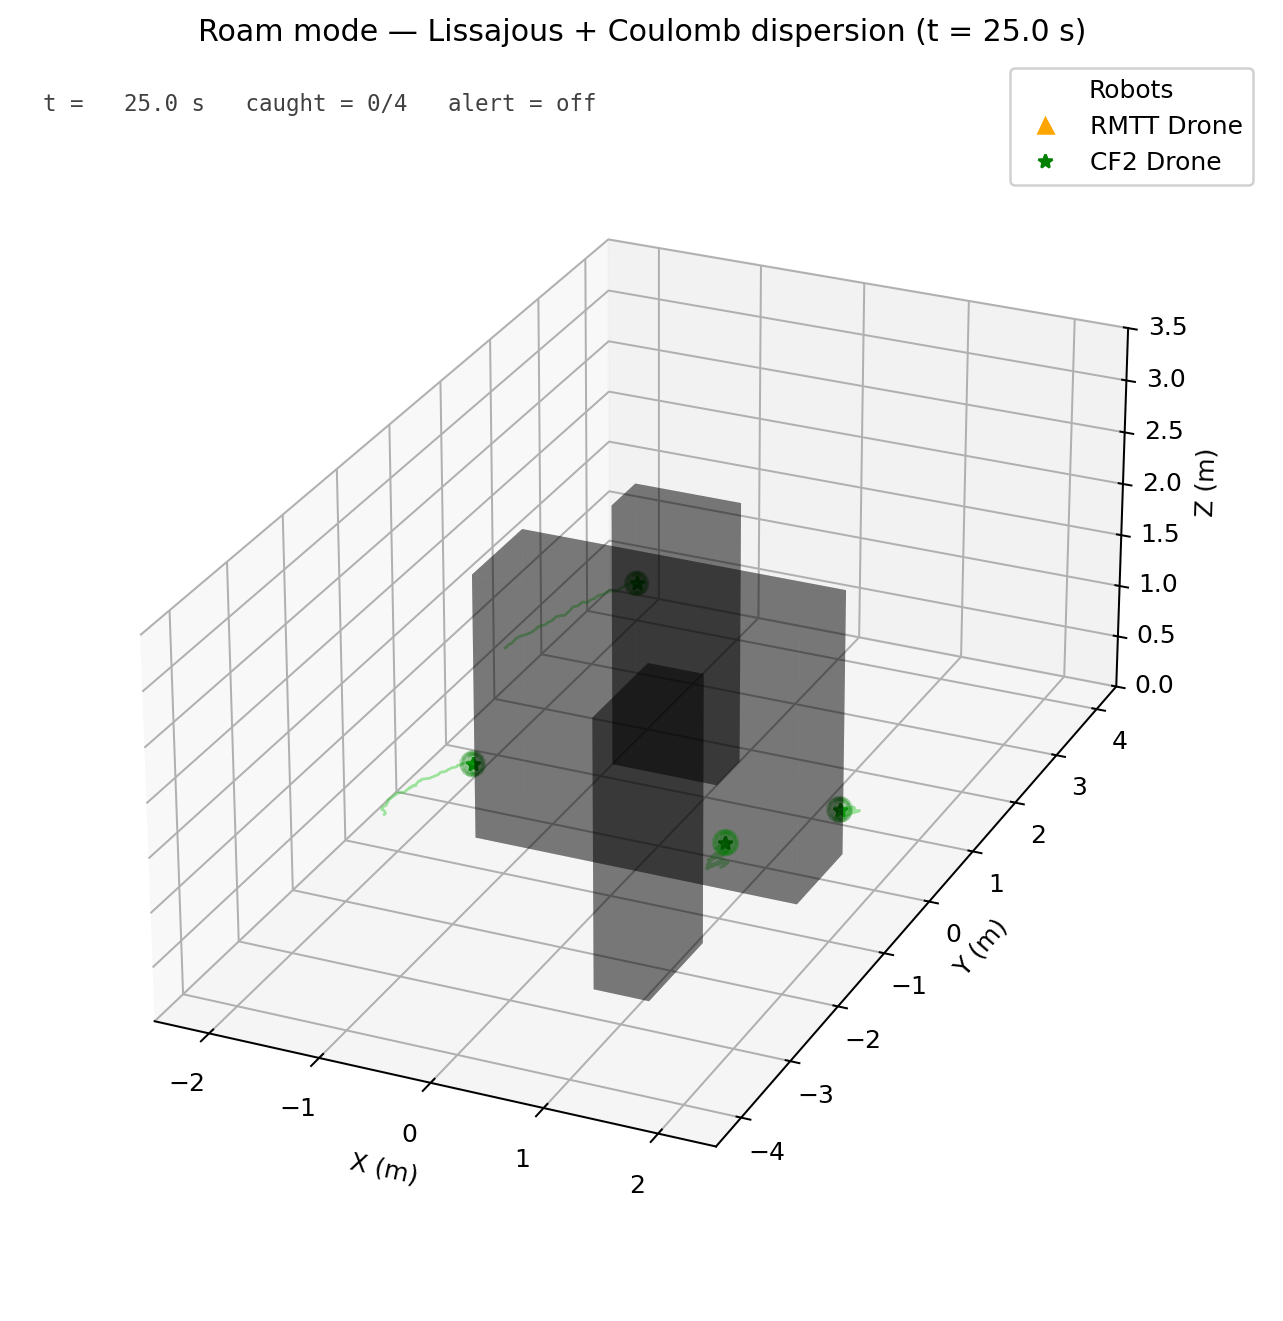
\includegraphics[width=0.80\linewidth]{figures/fig_roam_dispersion.png}
  \caption{Roam mode at $t = 25$\,s. With the seeker parked out of vision
  range, the swarm sits in its Coulomb-dispersion equilibrium inside the
  arena: hiders are pushed apart by $-\nabla V_\mathrm{disp}$, the boundary
  repulsion stops them from sticking to the walls, and the analytic
  Lissajous feed-forward keeps every hider drifting along its own quasi-orbit
  rather than freezing at a fixed point. Cones omitted to declutter the
  swarm geometry.}
  \label{fig:roam_dispersion}
\end{figure}

\subsection{Cover-assignment geometry (multi-agent)}
\label{sec:cover}

Hide mode is a small \emph{cooperative task-allocation} problem: there are
several cover spots and several hiders, and the swarm wants every hider on a
distinct spot so the seeker cannot harvest them in one cone sweep. The
solution lives in \code{cf2\_hider.assign\_cover\_targets} and runs in four
steps; the result is visualised in
Fig.~\ref{fig:hide_assignment} and Fig.~\ref{fig:hide_assignment_topdown}.

\paragraph{1. Candidate enumeration.}
For every obstacle (center $\vect{o}_j$, half-extents $(h_x, h_y)$) and every
AABB face with outward normal $\hat{\vect{n}} \in \{\pm\hat{\vect{e}}_x,
\pm\hat{\vect{e}}_y\}$, build the candidate
\[
    \vect{c}_{j,\hat{\vect{n}}}
    \;=\; \underbrace{\vect{o}_j + (\hat{\vect{n}} \cdot \vect{h})\,\hat{\vect{n}}}_{\text{face center}}
    + d_\mathrm{cov}\,\hat{\vect{n}}, \qquad d_\mathrm{cov} = 0.8\,\text{m},
\]
where $\vect{h} = (h_x, h_y)$. The face is \emph{kept} only if
$\hat{\vect{n}} \cdot (\vect{o}_j - \vect{s}) > 0$, i.e.\ the normal points
away from the seeker -- only those faces actually occlude line of sight to
the cover point. With the three obstacles of the default scenario, $3
\times 4 = 12$ candidates are generated before filtering; in a typical
seeker pose roughly half survive the directional gate. The
$d_\mathrm{cov} > r_\mathrm{safe}$ inequality is deliberate: the candidate
sits \emph{outside} the obstacle-consensus push zone, so a hider can come to
rest on it without fighting the avoidance law.

\paragraph{2. Cost matrix.}
With $N$ hiders and $M \ge N$ candidates, define
\(
    C_{ij} = \|\vect{p}_i^{xy} - \vect{c}_j\|_2^2.
\)
Squared distance gives the same min-cost solution as Euclidean distance and
avoids $N \cdot M$ square roots.

\paragraph{3. Min-cost injective assignment.}
Find $\pi : \{1,\dots,N\} \to \{1,\dots,M\}$ injective minimizing $\sum_i
C_{i,\pi(i)}$. For the default scenario $(N, M) \le (4, 12)$ the search space
is $P(M, N) \le 11{,}880$ permutations, so a branch-and-bound brute force is
faster and dependency-free compared to importing SciPy's
\code{linear\_sum\_assignment}. The implementation prunes any partial
assignment whose accumulated cost already exceeds the best complete one
(\code{cf2\_hider.\_best\_assignment}).

\paragraph{4. Hysteresis cache.}
The matching is \emph{not} recomputed every tick. A small cache
(\code{\_cover\_assignment\_cache}) stores the last solved assignment and
re-uses it as long as both of these hold:
\begin{itemize}[leftmargin=1.4em,topsep=2pt]
  \item \code{age} = $t - t_\mathrm{cache} < \code{\_COVER\_CACHE\_MAX\_AGE}
        = 1.0$\,s, and
  \item the seeker has moved less than
        \code{\_COVER\_CACHE\_SEEKER\_DELTA} $= 0.5$\,m since the cache was
        built.
\end{itemize}
Without this gate the cost matrix would shift slightly every tick on
position noise alone, occasionally swapping two hiders' assigned faces
when their costs cross -- a role swap that does not change the steady-state
formation but does send the affected pair on a wasted round-trip in the
meantime. The cache also drops the effective matching frequency from
$20$\,Hz to $\sim 1$\,Hz, which would matter on real flight hardware.

\paragraph{Decentralization.}
The simulator hands every hider the same \code{cf2\_poses} matrix and the
same shared seeker sighting; \code{assign\_cover\_targets} is deterministic
in those inputs and so is the cache. Every hider independently computes the
\emph{same} matching and reads its own row from the result -- a consensus
reached by ``every node solves the same optimization on the same inputs''
rather than by message exchange. No explicit communication is needed beyond
the existing shared-memory sighting channel.

\paragraph{Fallback.}
If $M < N$ (the seeker hides most far-side faces), the $N - M$ leftover
hiders fan out radially around the seeker at distance $1.5\,\text{m}$ on
angles $2\pi k / (N - M)$. They no longer get a true occlusion but they no
longer pile up either, and the dispersion consensus keeps pushing them
apart in the meantime. The single-target \code{seek\_cover\_target}
function (older nearest-cover-only behaviour) is kept exported for
backward compatibility and tests, but is no longer on the hot path.

\begin{figure}[htbp]
  \centering
  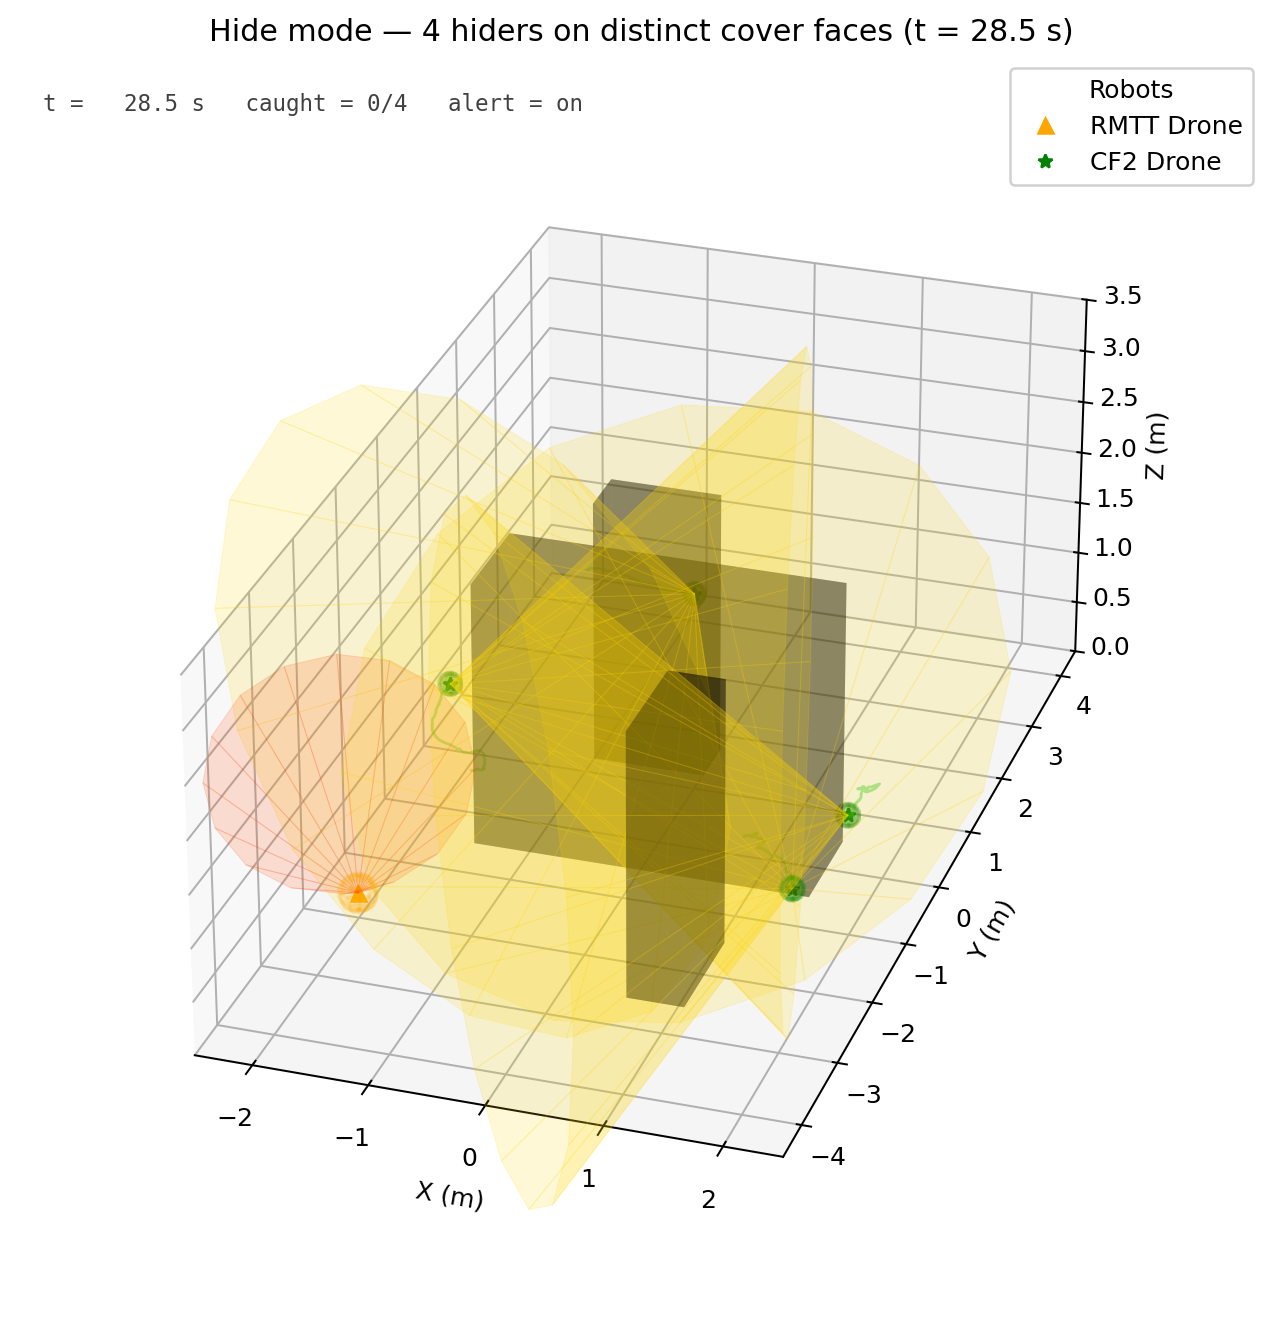
\includegraphics[width=0.78\linewidth]{figures/fig_hide_assignment.png}
  \caption{Hide mode (oblique 3D). The seeker has just emitted a sighting
  from $(0, -4, 0.8)$ (south wall, ahead of obstacle 2). The four hiders'
  cones switch to gold (alert), each hider has been assigned a distinct
  far-side cover face, and the swarm converges within $\sim 3$\,s
  (well inside the 5\,s TTL).}
  \label{fig:hide_assignment}
\end{figure}

\begin{figure}[htbp]
  \centering
  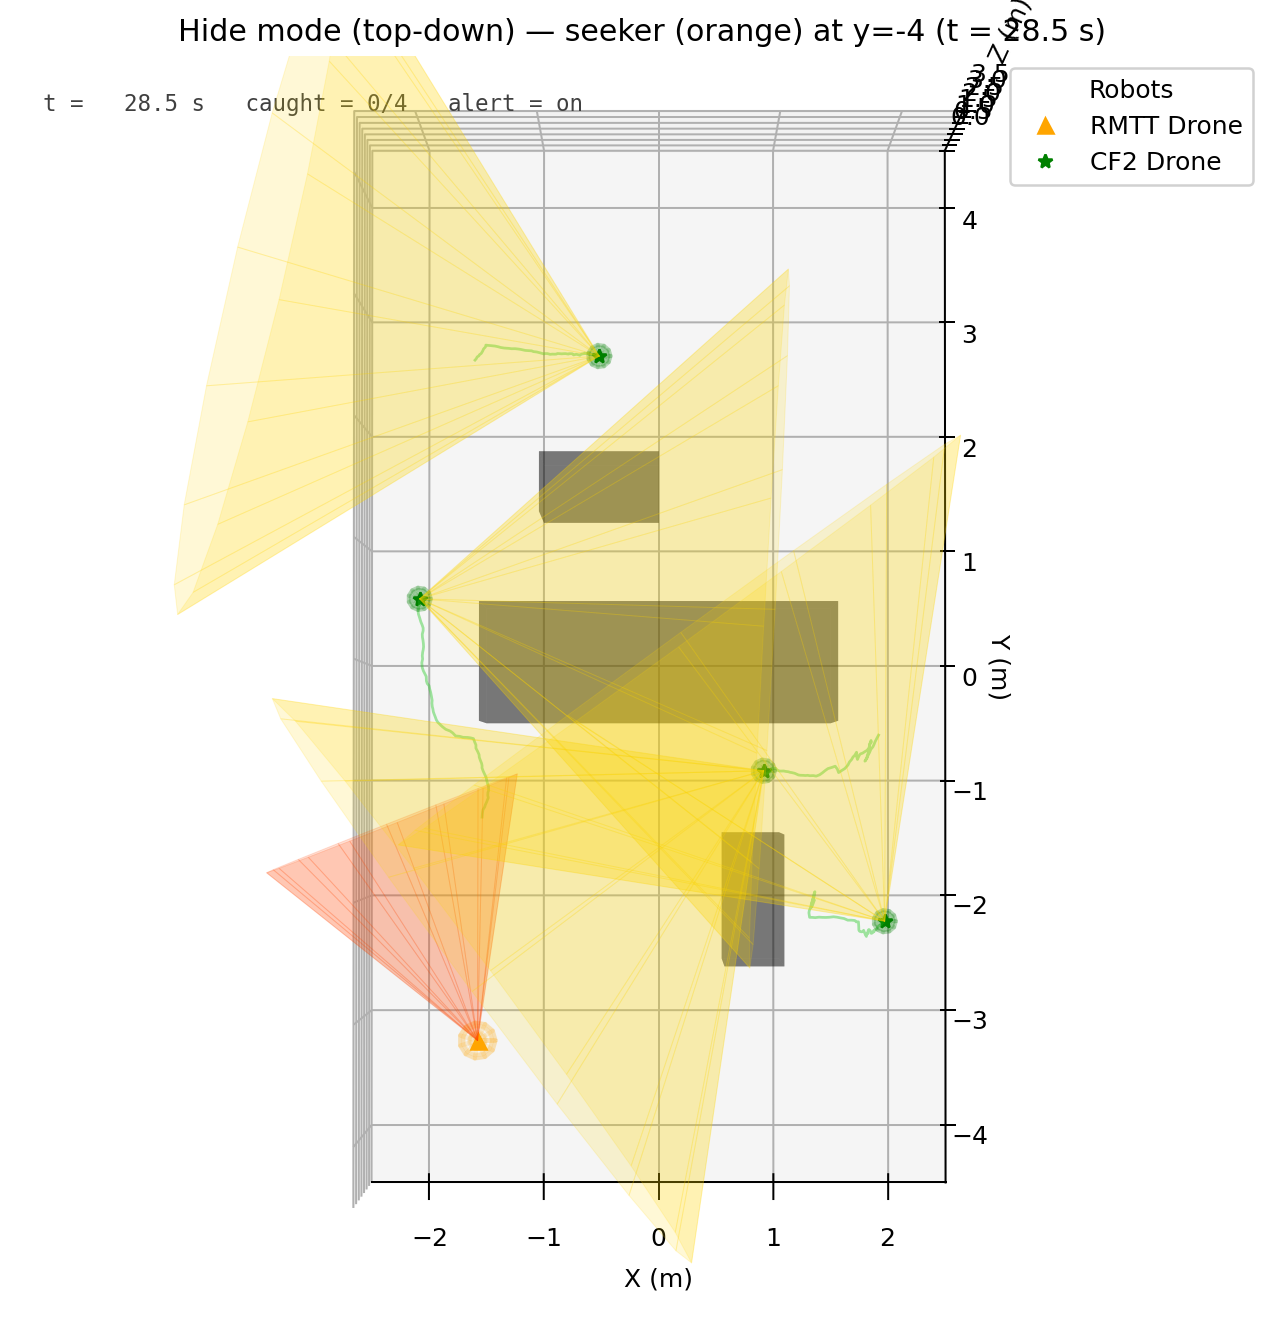
\includegraphics[width=0.62\linewidth]{figures/fig_hide_assignment_topdown.png}
  \caption{Same hide-mode instant viewed from straight above. Top-down makes
  the cover-face geometry unambiguous: each hider sits behind one obstacle
  face whose outward normal points \emph{away} from the seeker's south-side
  sighting, and no two hiders share a face -- the visual signature of the
  injective min-cost matching.}
  \label{fig:hide_assignment_topdown}
\end{figure}

% ============================================================
\section{Consensus laws (\code{cf2\_consensus.py})}
\label{sec:consensus}
% ============================================================

The module hosts two consensus laws used by the hiders. The obstacle
consensus (Sec.~\ref{sec:obs-consensus}) is also used by the seeker. The
inter-agent dispersion law (Sec.~\ref{sec:disp-consensus}) is hider-only and
is what gives the swarm its coordinated ``spread out'' behaviour.

\subsection{Obstacle consensus}
\label{sec:obs-consensus}
\subsubsection*{Definition}

Given a list of sensed obstacles, each with closest-surface distance $d_j$ and
outward normal $\vect{n}_j$, the consensus command is
\[
    \vect{u} \;=\; \sum_{j \,:\, d_j < r_\mathrm{safe}} \left[
                       k_\mathrm{obs}\,(r_\mathrm{safe} - d_j)
                     + k_\mathrm{bar}\!\left(\frac{r_\mathrm{safe}}{\max(d_j,\varepsilon)} - 1\right)
                   \right] \vect{n}_j.
\]
The function does \emph{not} saturate; saturation is the caller's
responsibility (the hider controller applies the magnitude cap on the summed
force, after adding the goal/separation/boundary contributions).

\subsubsection*{Properties}

\paragraph{Asymptotic (linear term).}
Define $e_j(\vect{p}) = \max(0, r_\mathrm{safe} - d_j(\vect{p}))$ and the
Lyapunov candidate
\[
    V(\vect{p}) \;=\; \tfrac{1}{2} \sum_j e_j(\vect{p})^2.
\]
For static obstacles, $\nabla d_j = \vect{n}_j$ on the violating set, so the
purely-linear closed loop $\dot{\vect{p}} = -k_\mathrm{obs}\sum_j e_j \vect{n}_j$
satisfies $\dot{V} = -k_\mathrm{obs}\sum_j e_j^2 \le 0$, with equality only when
all violations vanish. The drone therefore converges to the safe set $\{\vect{p}
: d_j(\vect{p}) \ge r_\mathrm{safe}\ \forall j\}$ -- an asymptotic consensus on
``be outside every safety bubble''.

\paragraph{Bounded actuation (barrier term).}
The linear term alone has bounded magnitude on bounded violations, so a
strong enough goal-attraction force could overpower it close to the obstacle.
The barrier term grows like $r_\mathrm{safe}/d_j$ as $d_j \to 0$, which
\emph{always} dominates any bounded attraction once the drone is close enough.
Combined with the actuator saturation in the caller, the closed-loop velocity
is bounded everywhere while the dynamics inside $\{d_j < r_\mathrm{safe}\}$
remain dominated by the avoidance push.

\paragraph{Numerical safety.}
The denominator uses $\max(d_j, \varepsilon)$ with
$\varepsilon = 0.02\,r_\mathrm{safe} = 12\,\text{mm}$. In simulation a drone may
briefly penetrate an obstacle due to the discrete integration step; this clamp
keeps the law finite while still producing a very large push.
Fig.~\ref{fig:barrier_curves} (left) shows the linear and barrier
components plotted side by side: the linear term carries all of the
restoring force at moderate violations while the barrier dominates as
$d \to 0$, exactly the property the controller relies on to remain
bounded under any bounded goal attraction.

\begin{figure}[htbp]
  \centering
  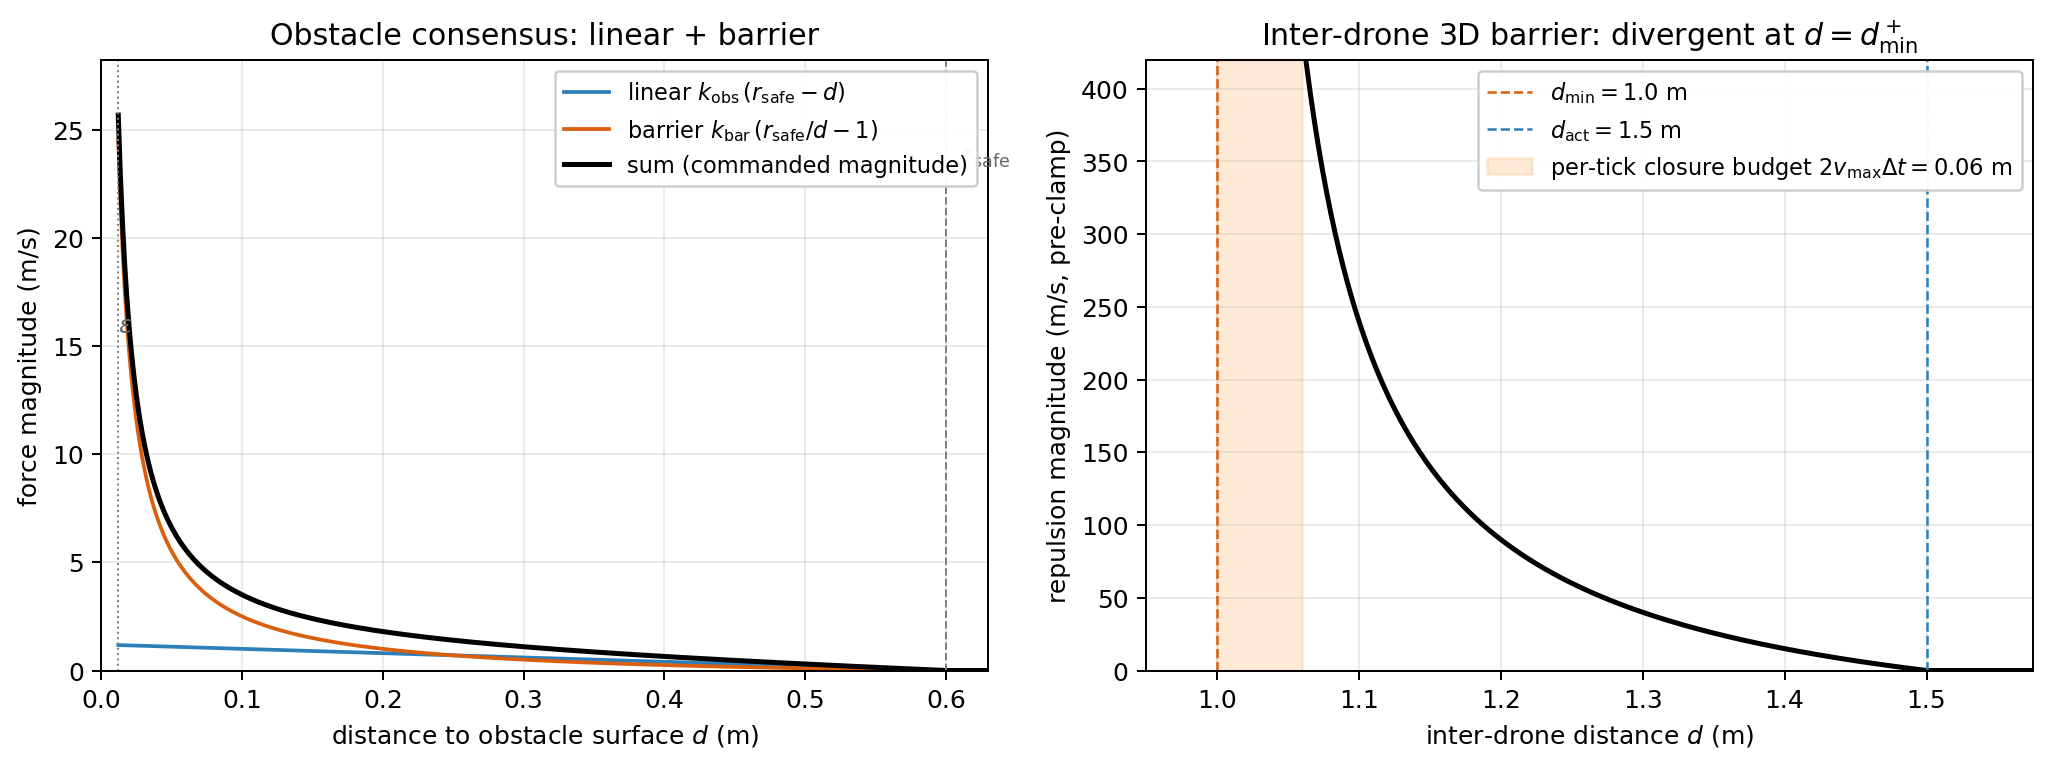
\includegraphics[width=0.97\linewidth]{figures/fig_barrier_curves.png}
  \caption{Left: obstacle consensus magnitude vs.\ distance to the obstacle
  surface, decomposed into the linear term $k_\mathrm{obs}(r_\mathrm{safe}
  - d)$ and the barrier term $k_\mathrm{bar}(r_\mathrm{safe}/d - 1)$. The
  numerical clamp at $\varepsilon = 0.02\,r_\mathrm{safe}$ caps the barrier
  at $\sim 25$\,m/s pre-saturation. Right: inter-drone 3D barrier
  magnitude vs.\ pairwise distance over the active band
  $[d_\mathrm{min}, d_\mathrm{act}]$. The shaded strip is the per-tick
  closure budget $2 v_\mathrm{max} \Delta t = 0.06$\,m -- the barrier is
  already in the hundreds of m/s by the time a relative-closure step could
  cross it, which underwrites the discrete-time invariance argument of
  Sec.~\ref{sec:tp-shim}.}
  \label{fig:barrier_curves}
\end{figure}

\subsection{Inter-agent dispersion consensus}
\label{sec:disp-consensus}

\subsubsection*{Definition}
For the hider swarm $\{\vect{p}_1, \dots, \vect{p}_N\} \subset \mathbb{R}^2$
(only the planar component enters the law), define the aggregate cost
\[
    V_\mathrm{disp}(\vect{p}_1, \dots, \vect{p}_N)
    \;=\; \frac{k_\mathrm{disp}}{2}
          \sum_{\substack{i, j \\ i \ne j}}
          \frac{1}{\|\vect{p}_i - \vect{p}_j\|}.
\]
Each hider runs the per-agent gradient descent
\[
    \vect{u}_i \;=\; -\nabla_{\vect{p}_i} V_\mathrm{disp}
    \;=\; k_\mathrm{disp} \sum_{j \ne i}
          \frac{\vect{p}_i - \vect{p}_j}{\|\vect{p}_i - \vect{p}_j\|^{3}}.
\]
This is the Coulomb form: agent $i$ feels an inverse-square push (in
\emph{magnitude} per unit charge) from every other agent. The
implementation floors $\|\vect{p}_i - \vect{p}_j\|$ at
$\varepsilon_\mathrm{disp} = 0.05\,\text{m}$ to keep the gradient bounded if
two hiders briefly co-locate.

\subsubsection*{Properties}

\paragraph{Aggregate Lyapunov.}
$V_\mathrm{disp}$ is itself a Lyapunov function for the joint flow
$\dot{\vect{p}}_i = \vect{u}_i$ on the unconstrained domain
$\{\vect{p}_i \ne \vect{p}_j \;\forall i \ne j\}$:
\[
    \dot{V}_\mathrm{disp}
    \;=\; \sum_i \nabla_{\vect{p}_i} V_\mathrm{disp} \cdot \dot{\vect{p}}_i
    \;=\; -\sum_i \|\nabla_{\vect{p}_i} V_\mathrm{disp}\|^2
    \;\le\; 0,
\]
with equality only at critical configurations of $V_\mathrm{disp}$. Every
hider's local descent decreases the \emph{same} swarm-level scalar -- the
defining property of a consensus law on an aggregate cost.

\paragraph{Long-range coupling.}
There is no cutoff: every other hider always contributes. Contrast with a
short-range repulsion (e.g.\ $1/d^2$ inside a 0.9\,m influence radius and
zero outside): such a law is silent the moment the swarm is more than
0.9\,m apart, so it cannot push two well-separated hiders further apart.
The Coulomb form pushes at any distance, so the equilibrium is determined
by the boundary and obstacle constraints, not by the law going silent.

\paragraph{Centroid invariance and bounded equilibria.}
$\vect{F}^{(j \to i)}_\mathrm{disp} = -\vect{F}^{(i \to j)}_\mathrm{disp}$
(Newton's third law in form), so the swarm centroid is invariant under
$\vect{F}_\mathrm{disp}$ alone. Bounded equilibria emerge from the
combination with the boundary repulsion of Sec.~\ref{sec:disp-force}: the
walls confine the swarm to the arena while $\vect{F}_\mathrm{disp}$
pushes the hiders to the configuration with maximum pairwise distances
inside that confinement.

\paragraph{Decentralization.}
The law uses only $\vect{p}_i$ and $\{\vect{p}_j\}_{j \ne i}$ -- the
simulator-provided pose matrix is the only neighbourhood query needed, no
extra messaging. In a real deployment the assumed information flow is
``each hider broadcasts its position to all the others at controller
frequency''. The shared-memory channel already exists for seeker sightings
(Sec.~\ref{sec:cover}) and would extend trivially to position broadcasts.

\begin{figure}[htbp]
  \centering
  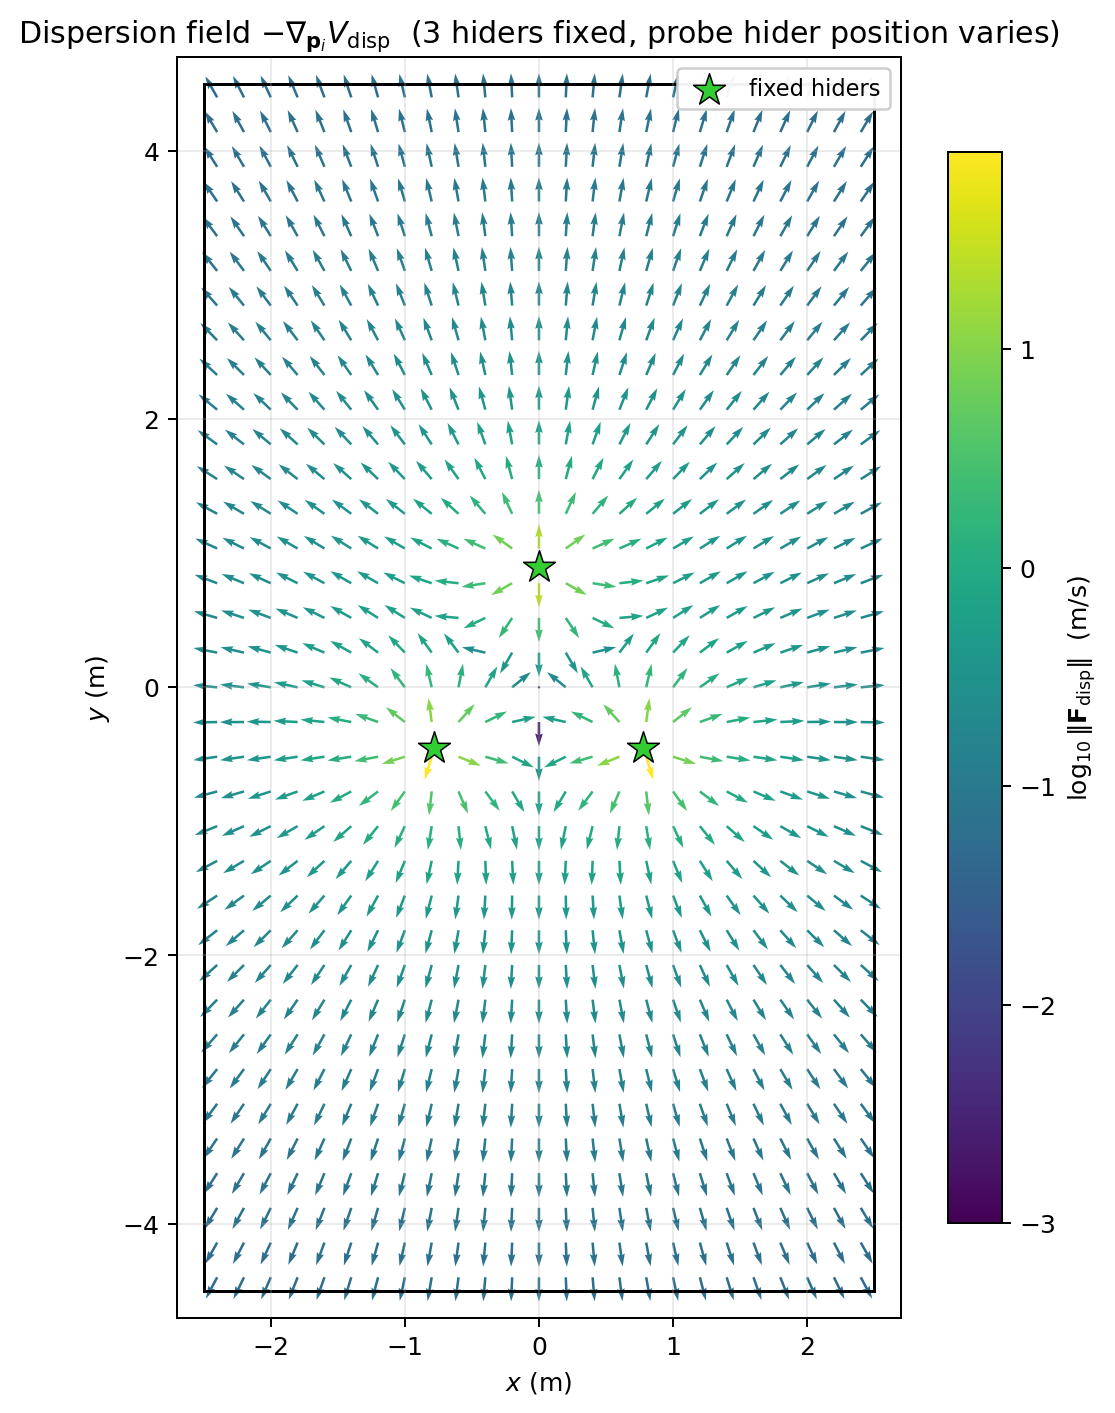
\includegraphics[width=0.62\linewidth]{figures/fig_dispersion_field.png}
  \caption{Dispersion field $-\nabla_{\vect{p}_i} V_\mathrm{disp}$ for a
  probe hider at every grid point, with three other hiders held fixed at
  the marked positions. Arrow direction shows the per-tick velocity
  command; colour shows its $\log_{10}$ magnitude. The field is radial-out
  from each fixed neighbour and never goes silent at any distance, which
  is exactly the property a short-range repulsion would lack.}
  \label{fig:dispersion_field}
\end{figure}

\begin{figure}[htbp]
  \centering
  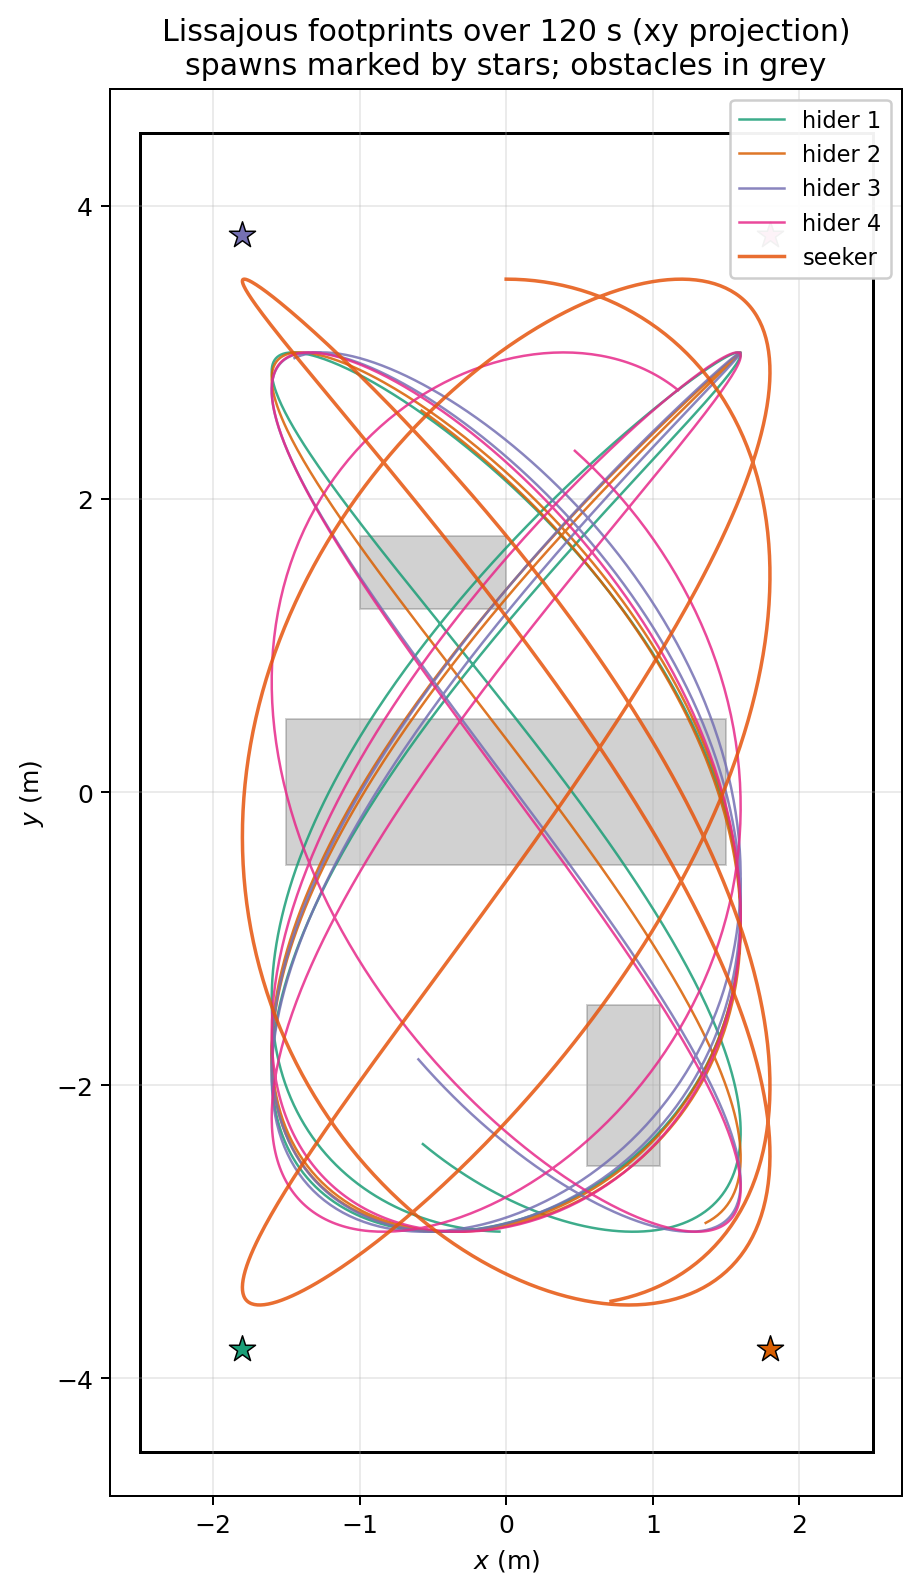
\includegraphics[width=0.55\linewidth]{figures/fig_lissajous_footprint.png}
  \caption{Lissajous footprints over $120$\,s ($xy$ projection). Each
  hider's path uses its individual frequency/phase offsets and the lazy
  initial-phase offset $\tau_i$ described in Sec.~\ref{sec:lissajous}; the
  spawns (stars) lie on each curve by construction. The seeker's
  slow figure-of-eight is drawn in orange. The three obstacle footprints
  are overlaid in grey -- note that the Lissajous orbits cross the obstacle
  AABBs, which is why the obstacle consensus must remain active even when
  the goal is supposedly on the safe side.}
  \label{fig:lissajous_footprint}
\end{figure}

% ============================================================
\section{Sensing (\code{cf2\_sensing.py})}
% ============================================================

\subsection{Intent heading}

The heading used both for the FoV cone and the sensing axis is the unit vector
toward the current Lissajous target:
\[
    \hat{\vect{h}}(t)
    \;=\;
    \frac{\vect{p}_\mathrm{lis}(t) - \vect{p}(t)}{\|\vect{p}_\mathrm{lis}(t) - \vect{p}(t)\|},
    \qquad \text{with}\ dz \mathrel{\!:=\!} 0
    \ \text{forced before normalization.}
\]
Compared to a path-tangent heading
$\dot{\vect{p}}_\mathrm{lis}/\|\dot{\vect{p}}_\mathrm{lis}\|$, this points
where the drone wants to be rather than where the path is currently
moving. The practical consequence: when an obstacle is between the drone
and its waypoint, the cone is already aimed at the obstacle. The forced
$dz = 0$ (\code{cf2\_sensing.py:38}) is part of the disabled-Z policy of
Sec.~\ref{sec:lissajous}: the heading is a unit vector in the $xy$ plane,
and so the rendered cone is a 2D wedge embedded in 3-space.

\subsection{FoV-cone obstacle sensing}

For each obstacle $\mathcal{B}_j$, the function \code{sense\_obstacles}:
\begin{enumerate}[leftmargin=1.4em]
  \item Computes the closest box point $\vect{c}_j$ to the drone (per-axis
        clamp).
  \item Computes the 3D distance $d_j = \|\vect{c}_j - \vect{p}\|$ and rejects
        the obstacle if $d_j > $ \code{sensing\_radius}.
  \item Applies the angular gate $\hat{\vect{h}} \cdot \hat{\vect{e}}_j \ge
        \cos\theta_\mathrm{fov}$ where $\hat{\vect{e}}_j = (\vect{c}_j -
        \vect{p})/d_j$, returning the obstacle's $\vect{n}_j = -\hat{\vect{e}}_j$
        and $d_j$.
\end{enumerate}

A degenerate case is handled explicitly: if $d_j < 10^{-6}$ (drone is on or
inside the obstacle) the function flags it as in-cone with $\vect{n}_j =
-\hat{\vect{h}}$, so the downstream consensus law pushes the drone back along
the inverse of its heading.

\paragraph{Why hiders sense omnidirectionally.}
The hider controller passes $\theta_\mathrm{fov} = \pi$ to
\code{sense\_obstacles}, effectively disabling the angular gate. The forward
$45^\circ$ cone is reserved for \emph{seeker detection}, not obstacle
avoidance, since otherwise a hider would be free to enter an obstacle from a
blind side. Like the heading, the obstacle-cone test forces $dz = 0$ in the
delta to the closest box point (\code{cf2\_sensing.py:88}); since the cone
test is omnidirectional for the hider this is moot in practice, but the
same code path is reused (with a real cone) by the seeker -- a small bit of
asymmetry that should be tightened up if Z is re-enabled.

\begin{figure}[htbp]
  \centering
  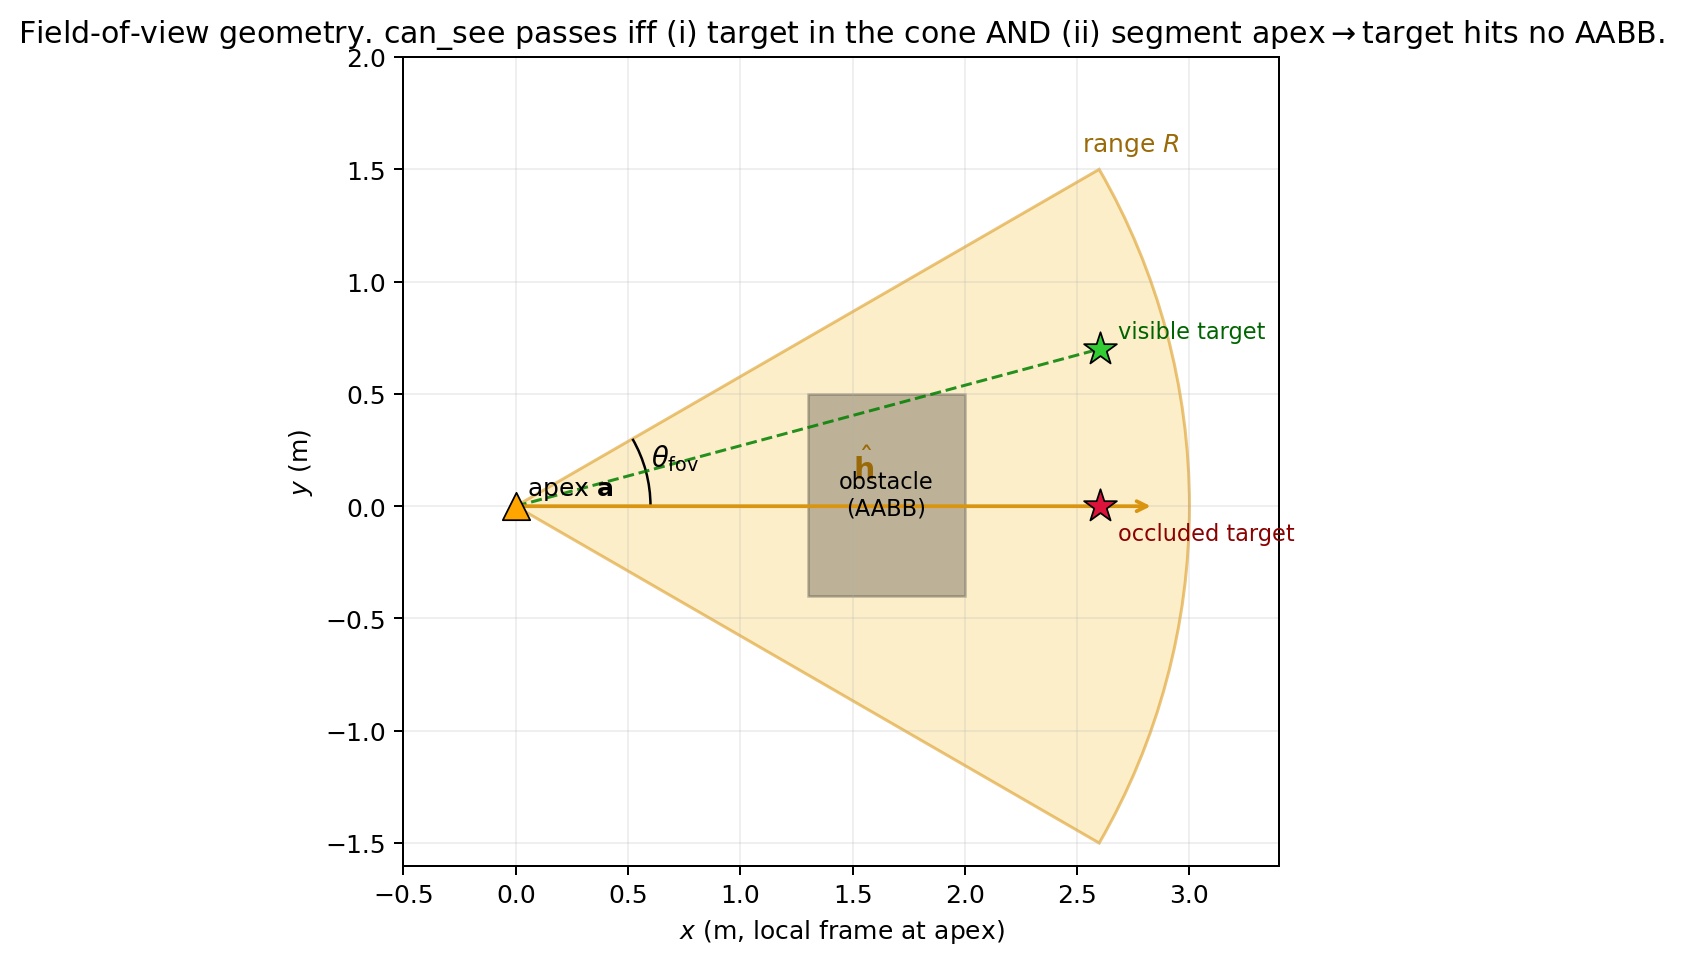
\includegraphics[width=0.85\linewidth]{figures/fig_fov_geometry.png}
  \caption{Geometry of \code{can\_see} (\code{rmtt\_seeker.py:153}). The
  predicate is true iff the target lies inside the cone (range and
  angular gates both pass) \emph{and} the segment from apex to target
  intersects no AABB obstacle. The Kay--Kajiya slab algorithm
  (\code{\_segment\_intersects\_aabb}) performs the per-axis interval
  intersection that decides occlusion.}
  \label{fig:fov_geometry}
\end{figure}

% ============================================================
\section{Seeker controller (\code{rmtt\_seeker.py})}
% ============================================================

\subsection{Sweep path}
The seeker tracks a slow Lissajous sweep:
\[
    \vect{p}_\mathrm{goal}^{S}(t) = \begin{pmatrix}
        A_X^S \sin(\Omega_X t) \\
        A_Y^S \sin(\Omega_Y t + \pi/2) \\
        c_z^S + A_Z^S \sin(\Omega_Z t)
    \end{pmatrix},
\]
with $A_X^S = 1.8$, $A_Y^S = 3.5$, $A_Z^S = 0$ (Z disabled, same scaffolding
story as the hider in Sec.~\ref{sec:lissajous}), $c_z^S = \code{RMTT\_HOVER\_Z}
= 0.8$\,m, and angular frequencies $\Omega_X = 0.18$, $\Omega_Y = 0.13$,
$\Omega_Z = 0.08$ rad/s. $\Omega_Z$ is kept for symmetry with the $x, y$
branch but is multiplied by $A_Z^S = 0$ so produces no motion. Cycle times
are $\approx 35$ and $48\,\text{s}$. The $\pi/2$ phase between $x$ and $y$
produces a figure-of-eight footprint that sweeps both ``rooms'' of the arena
every full cycle (overlaid in Fig.~\ref{fig:lissajous_footprint}).

\paragraph{Why the seeker hovers below the hiders.}
$c_z^S = 0.8$\,m is intentionally below the hiders' $1.0$\,m cruise. Even
though the seeker's own heading is computed with $dz = 0$
(\code{rmtt\_seeker.py:71}), the cone test in \code{can\_see} is fully 3D
(\code{rmtt\_seeker.py:158}). The $0.2$\,m altitude offset together with the
$30^\circ$ half-angle means a hider directly overhead is already $11^\circ$
off-axis -- not a free catch, but a meaningful geometric constraint that
makes the catch easier when the seeker is closer in $xy$.

\subsection{Control law}
The seeker uses the same obstacle consensus law as the hiders (with the
same parameters $r_\mathrm{safe} = 0.6$, $k_\mathrm{obs} = 2$,
$k_\mathrm{bar} = 0.5$) plus a goal attraction
$\vect{F}_\mathrm{goal}^S = k_g^S (\vect{p}_\mathrm{goal}^S - \vect{p})$ with
$k_g^S = 0.8$, and the soft boundary repulsion of Sec.~\ref{sec:seeker-bnd}.
The xy magnitude is saturated at $v_{\max,xy}^S = 0.6$\,m/s; the vertical
component is clipped to $|v_z^S| \le 0.6$\,m/s (the same value, so there is
no separate vertical cap any more) and then the simulator's
\code{clamp\_vel3d} applies the unified 3D actuator clamp at
$\text{MAX\_V\_RMTT} = 0.6$\,m/s.

The signature \code{compute\_seeker\_cmd(robot\_no, robot\_pose,
obstacle\_pose, obstacle\_size, clock)} deliberately does \emph{not} accept
hider positions: the seeker's \emph{navigation} cannot use any hider state.
The \code{tp\_algos.rmtt\_control\_fn} wrapper does receive \code{cf2\_poses}
(its signature is fixed by the TP framework) and uses them \emph{only} to add
the 3D safety-fence repulsion of Sec.~\ref{sec:tp-shim} -- it never forwards
them to \code{compute\_seeker\_cmd}, so the controller's planning logic
remains hider-blind. The same wrapper is what notices when \code{catch\_count()
$\ge$ nbCF2} and sets the seeker's \code{trigger\_land} flag, ending the
game; the seeker controller itself has no game-state input.

\subsection{Soft boundary repulsion}
\label{sec:seeker-bnd}
Unlike the hider, the seeker has no inter-agent dispersion term pulling it
inward, only its goal attraction toward the centred Lissajous target. On
the slowest axis ($\Omega_Y$) the cycle is $48$\,s and the path swings to
$|y| = 3.5$\,m near the wall at $|y| = 4.5$; under unmodelled drift this is
close enough that the simulator's 3D clamp can occasionally graze the
boundary. The fix (added in commit \code{a68365d}) is a soft $1/d$
repulsion of the same form as the hider's (Sec.~\ref{sec:lissajous}):
\[
    F_\mathrm{bnd}^{S,(w)} \;=\; g_\mathrm{bnd}^S
    \!\left(\frac{1}{\max(d,10^{-4})} - \frac{1}{m^S}\right),
    \qquad m^S = 0.6,\ g_\mathrm{bnd}^S = 0.3.
\]
The gain $g_\mathrm{bnd}^S = 0.3$ is $3.3\times$ the hider's $0.09$ -- the
hider's wall push is a gentle nudge that the dispersion can easily
over-power, while the seeker's wall push has to do the entire restoring
job on its own.

\subsection{Search cone and line-of-sight}

The search cone has half-angle $\theta_\mathrm{seek} = 30^\circ$ and range
$\code{SEEKER\_VISION\_RANGE} = 2.0$\,m -- narrower than the hider's cone,
and \emph{shorter} (earlier experimental builds with a $3.5$\,m range caught
every hider within a single sweep; reducing the range to $2.0$\,m is what
finally made the game winnable for the hiders, because they detect the
seeker at $3.0$\,m and thus have a $\sim 1$\,m head-start to commit to
hide mode before they can be tagged). The predicate
\code{can\_see(apex, target, heading, fov\_half, range, obstacles)} returns
\code{True} when:
\begin{enumerate}[leftmargin=1.4em]
  \item The 3D distance $\|\vect{t} - \vect{a}\| \le$ range.
  \item The cone condition holds: $(\vect{t} - \vect{a}) \cdot \hat{\vect{h}}
        \ge \cos\theta_\mathrm{fov}\,\|\vect{t} - \vect{a}\|$.
  \item No obstacle box intersects the line segment from apex to target.
\end{enumerate}
A concrete catch event captured at simulator level is shown in
Fig.~\ref{fig:catch_moment}.

The occlusion test uses the standard Kay--Kajiya slab algorithm
(\code{\_segment\_intersects\_aabb}): for each of the 3 axes, compute the
parameter interval $[t_1, t_2]$ over which the segment lies between the slab
faces; intersect the three intervals; the segment hits the box iff the
intersection overlaps $[0, 1]$. Axis-parallel segments are handled with an
explicit ``inside the slab?'' check.

\begin{figure}[htbp]
  \centering
  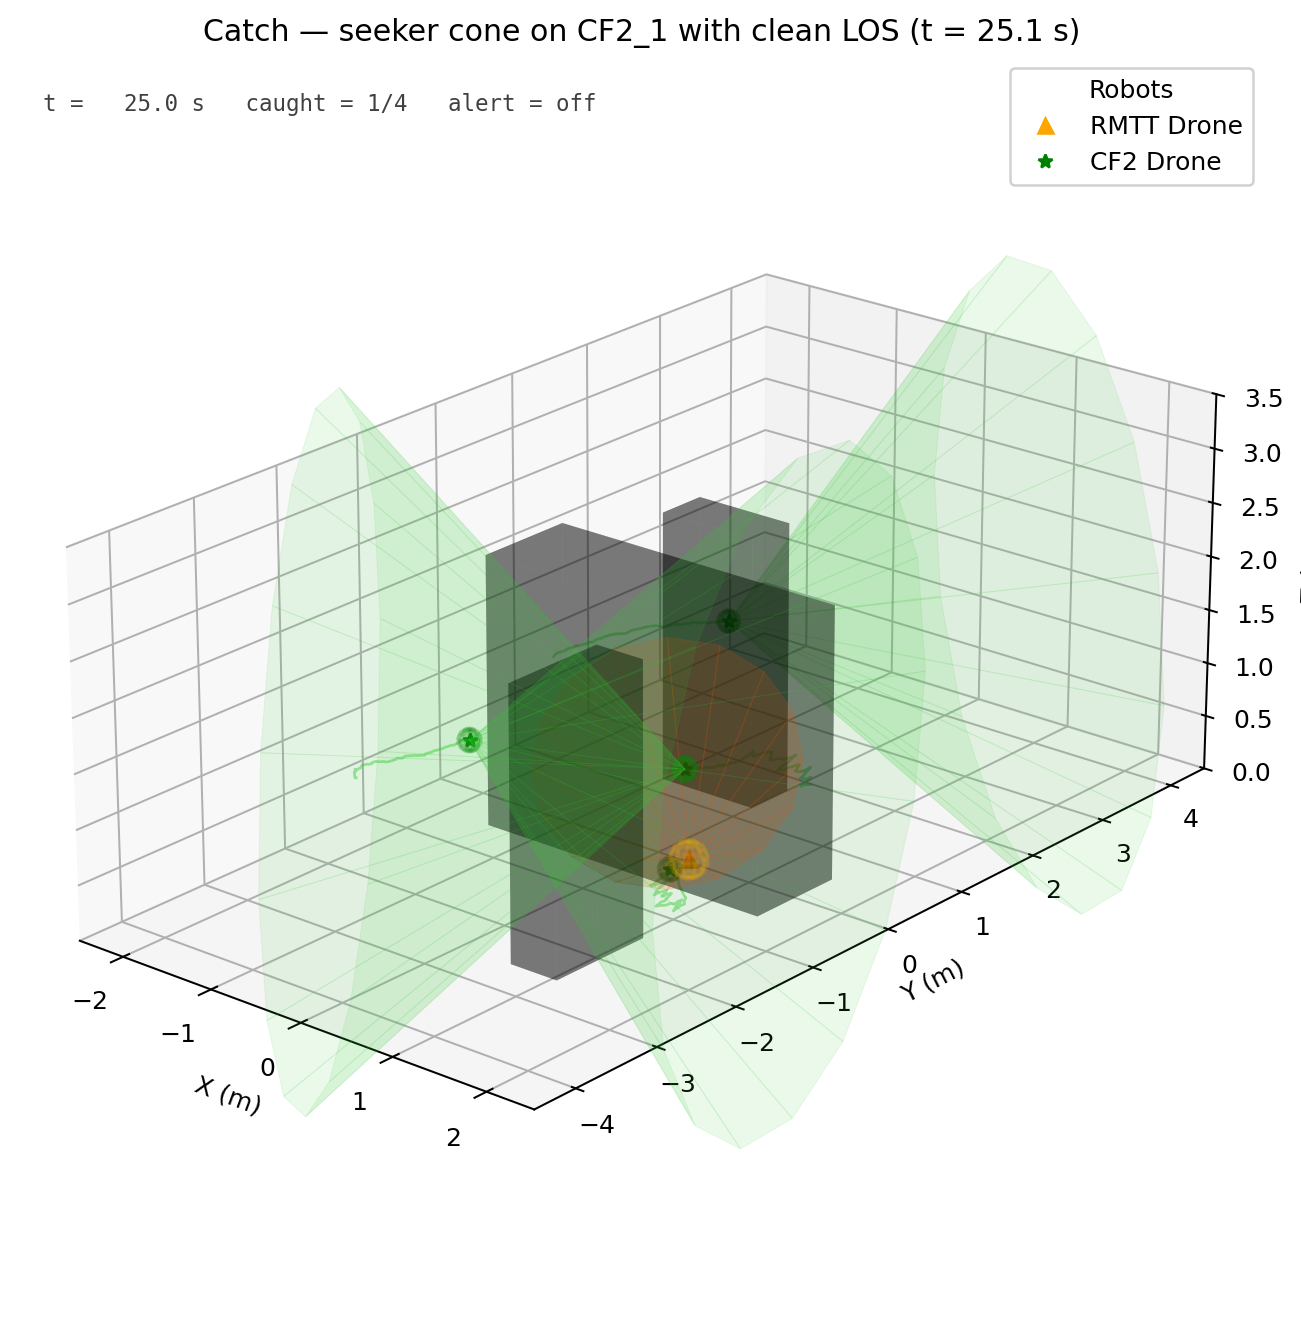
\includegraphics[width=0.78\linewidth]{figures/fig_catch_moment.png}
  \caption{Deterministic catch event. The seeker is positioned $1.4$\,m
  south-east of CF2\_1 with the cone axis forced toward the hider; the
  Kay--Kajiya occlusion test passes (no AABB intersects the segment);
  \code{game\_referee.update\_catches} marks the hider on the next tick;
  and the hider's controller sees \code{is\_caught(1) = True} and switches
  to \code{trigger\_land = True} (LED red).}
  \label{fig:catch_moment}
\end{figure}

% ============================================================
\section{Inter-hider communication (\code{cf2\_hider.py})}
% ============================================================

The shared state is a single module-level dict:
\begin{lstlisting}
_last_seen = {'position': None, 'timestamp': None}
SEEKER_MEMORY_TTL = 5.0  # seconds
\end{lstlisting}
Writers (\code{report\_seeker\_sighting}) overwrite both fields atomically;
readers (\code{get\_last\_seen}) compare \code{t - timestamp} against the TTL
and return either the position or \code{None}. Last-write-wins is fine here
because the question is ``what is the most recent fix on the seeker'', and
between two sightings the older one offers no extra information.

\paragraph{TTL choice.}
$5\,\text{s}$ is enough to keep the swarm in hide mode for several controller
cycles after a sighting (the cover-assignment step is itself updated every
tick, so the swarm reshuffles quickly inside the window), yet much shorter
than a full seeker sweep, so the hiders return to dispersion-driven roaming
soon after the threat leaves sight. The exact value is not critical: a
shorter TTL biases the swarm toward exploration (more dispersion, less time
spent in cover), a longer one biases it toward defence.

\paragraph{Threading.}
The simulator runs each controller in a \code{ThreadPoolExecutor}. Python's
GIL plus the atomic-dict-write convention is enough here: a reader can never
see a half-written record, only a fully old or fully new one.

% ============================================================
\section{Catch detection (\code{game\_referee.py})}
% ============================================================

The referee owns a \code{set} of caught hider IDs and a dict of catch times.
Each frame it iterates over (flying seekers) $\times$ (flying, not-yet-caught
hiders), calls \code{can\_see} (the same predicate the seeker would compute
internally if it had one), and adds the hider to the caught set if visible.
Once caught, a hider stays caught for the rest of the simulation. The
hider controller in \code{tp\_algos.cf2\_control\_fn} reads this flag via
\code{is\_caught(robot\_no)} and returns \code{trigger\_land = True}, which
puts the drone into landing state.

\paragraph{End-of-game: the seeker lands too.}
The seeker wrapper in \code{tp\_algos.rmtt\_control\_fn} polls
\code{catch\_count()} every tick; when it reaches \code{nbCF2} (all hiders
caught), it short-circuits the call to \code{compute\_seeker\_cmd}, emits
$(0, 0, 0)$ as the velocity command, and sets \code{trigger\_land = True}
(lines 275--279). The simulator then drives the seeker through its state-3
landing transient (linear descent over \code{LANDING\_TIME = 3}\,s, same
as the takeoff except in reverse) and returns it to idle. The referee's
\code{\_caught} set persists for the module's lifetime, so re-takeoff in
the same Python process replays a frozen game state -- a minor wart that
is flagged in Future Work.

\begin{figure}[htbp]
  \centering
  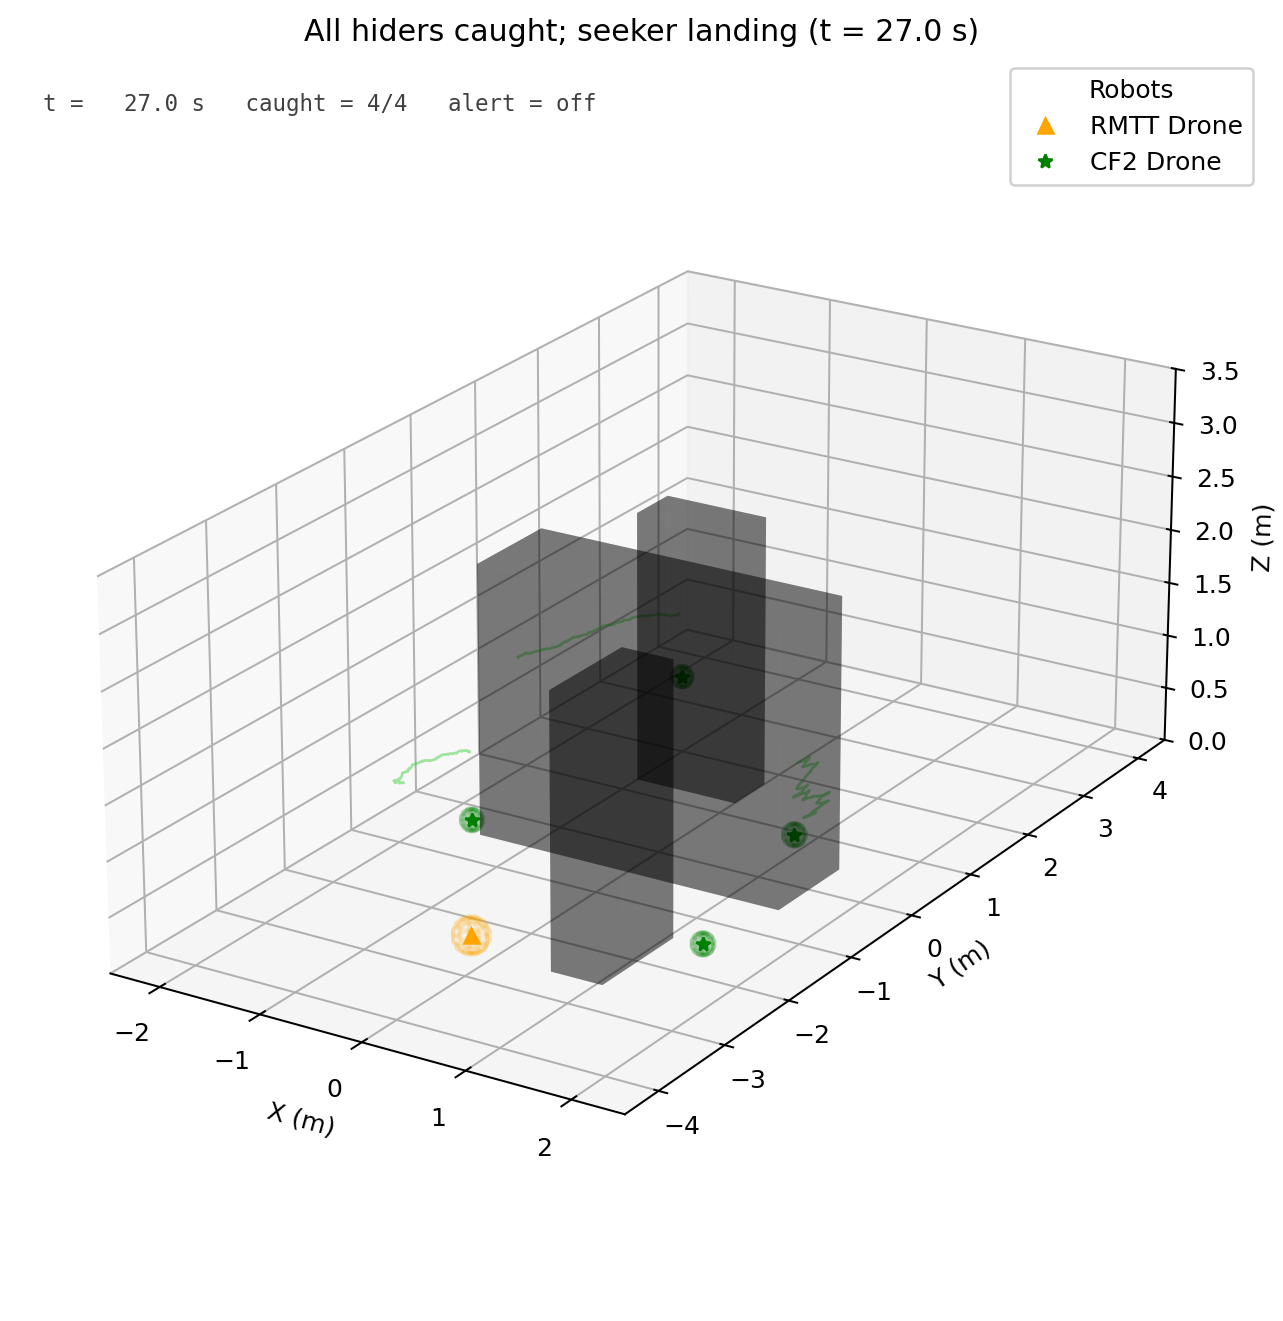
\includegraphics[width=0.78\linewidth]{figures/fig_end_game.png}
  \caption{End of game: \code{catch\_count() = 4/4}. The four hiders have
  triggered \code{trigger\_land} and are descending or already on the
  floor; the seeker has entered its own state-3 landing transient and is
  cruising downward in place. The HUD shows the final state.}
  \label{fig:end_game}
\end{figure}

% ============================================================
\section{Visualization (\code{sim\_viz.py})}
% ============================================================

The visualization layer adds three things on top of the simulator's basic
markers:
\begin{itemize}[leftmargin=1.4em]
  \item \textbf{3D FoV cones.} For each flying drone, a triangle-fan
        polyhedron is built with apex at the drone and axis along its
        heading. The 16-segment base disk is constructed in the plane
        perpendicular to the heading using an orthonormal basis built from
        an arbitrary reference vector (world-$z$, switching to world-$x$
        when the heading is nearly vertical). The heading the cone uses is
        \code{hider\_view\_heading} for hiders and \code{seeker\_heading}
        for the seeker; in the hider case this is the \emph{same} function
        the controller passes to \code{can\_see}, so the on-screen cone and
        the cone that actually triggers a sighting are guaranteed to
        coincide (see Sec.~\ref{sec:cover}, ``One heading function for
        both vision and rendering'').
  \item \textbf{Position trails.} Each hider keeps a bounded deque
        (\code{TRAIL\_LEN = 80}) of recent positions, drawn as a thin green
        line. When the hider returns to idle (after a catch landing) the
        trail is cleared so the next takeoff starts fresh.
  \item \textbf{HUD.} A small monospace text in the upper left shows
        $t$, the catch count, and an \code{alert on/off} flag derived from
        \code{get\_last\_seen(t)}.
\end{itemize}
The cone colour for the hiders switches from \code{limegreen} (roam) to
\code{gold} (alert) when a fresh sighting is in shared memory, so the global
mode is visible at a glance.

% ============================================================
\section{Simulator hooks and controller-level separation (\code{tp\_algos.py})}
\label{sec:tp-shim}
% ============================================================

The TP framework requires every controller to live in \code{tp\_algos.py}
with a fixed signature. Per the project rules, only the body marked
\code{TO BE MODIFIED} may be edited. Two responsibilities live here:
\begin{enumerate}[leftmargin=1.4em]
  \item Dispatch each robot type to its dedicated module
        (\code{cf2\_milestone1}, \code{rmtt\_seeker}, \dots).
  \item Apply a controller-level 3D drone-to-drone separation \emph{on top of}
        what each module returns. This is the only place in the code base
        that has simultaneous access to \emph{both} hider and seeker poses, so
        it is the natural place to enforce a global ``no two drones get
        closer than 1\,m'' rule.
\end{enumerate}

\subsection{3D inter-drone barrier: a hard 1\,m floor}

\code{\_compute\_drone\_repulsion\_3d(self\_pose, neighbors,
min\_dist=1.0, activation=1.5)} enforces a \emph{hard} minimum separation
$d_\mathrm{min} = 1\,\text{m}$ between any pair of drones (hider-hider and
hider-seeker alike). For each neighbor $k$ with $d_{ik} < d_\mathrm{act}$:
\[
    \Delta\vect{v}_i \;=\; g_\mathrm{rep}
    \sum_{k\,:\,d_{ik} < d_\mathrm{act}}
    \!\left(\frac{1}{d_{ik} - d_\mathrm{min}} - \frac{1}{d_\mathrm{act} - d_\mathrm{min}}\right)
    \frac{\vect{p}_i - \vect{p}_k}{\|\vect{p}_i - \vect{p}_k\|},
    \quad g_\mathrm{rep} = 30,\ d_\mathrm{act} = 1.5\,\text{m}.
\]
The magnitude vanishes continuously at $d = d_\mathrm{act}$ and diverges as
$d \to d_\mathrm{min}^+$. If a pathological state $d \le d_\mathrm{min}$ is
ever observed (e.g.\ at spawn), the function returns a $10^6$-magnitude
outward command which, after the simulator's per-axis clamp at
$\text{MAX\_V} = 0.6\,\text{m/s}$, drives the drone at full speed purely
outward.

\paragraph{Discrete-time non-penetration argument.}
Let $\Delta t = 0.05\,\text{s}$ and $v_\mathrm{max} = 0.6\,\text{m/s}$.
The largest closure two drones can produce in one tick is
$2 v_\mathrm{max} \Delta t = 0.06\,\text{m}$. Suppose at tick $k$ we have
$d_k > d_\mathrm{min}$.
\begin{itemize}[leftmargin=1.4em]
  \item If $d_k \ge d_\mathrm{act}$, the barrier is zero on this step but
        $d_{k+1} \ge d_k - 0.06 \ge d_\mathrm{act} - 0.06 = 1.44\,\text{m}
        > d_\mathrm{min}$.
  \item If $d_\mathrm{min} < d_k < d_\mathrm{act}$, the barrier magnitude
        already exceeds the controllers' bounded xy commands ($\le
        0.45\,\text{m/s}$ for the hider, $\le 0.55\,\text{m/s}$ for the
        seeker) once $d_k \le d_\mathrm{act} - 0.06$. The clamp therefore
        resolves the net velocity to $v_\mathrm{max}$ purely outward on
        both drones, and
        $d_{k+1} \ge d_k + 2 v_\mathrm{max} \Delta t > d_\mathrm{min}$.
\end{itemize}
Combining the two cases, $d_k > d_\mathrm{min} \Rightarrow d_{k+1} >
d_\mathrm{min}$ for every $k$. The 1\,m floor is invariant under the
closed-loop dynamics.

A numerical degenerate case ($d_{ik} < \varepsilon = 10^{-6}$\,m) returns a
fixed $+x$ push so the function never divides by zero. The sum operates in
all three axes, contrary to the planar dispersion consensus in
\code{cf2\_milestone1} which only sees $xy$; the 3D component matters when a
hider and the seeker happen to be vertically aligned (which the dispersion
law ignores by construction). The two laws compose by addition, so the
barrier acts as a short-range 3D hard fence on top of whatever long-range
$xy$ geometry the dispersion law has chosen.

\subsection{How the helper is used}

\begin{itemize}[leftmargin=1.4em]
  \item \code{cf2\_control\_fn}: once the hider is flying and is not caught,
        it calls \code{compute\_roaming\_cmd} for $(v_x, v_y, z_\mathrm{dist},
        \text{led})$. It then collects \emph{all other} flying CF2s
        \emph{and all} RMTT seekers as neighbors, asks
        \code{\_compute\_drone\_repulsion\_3d} for $(\Delta v_x, \Delta v_y,
        \Delta v_z)$, and adds the result to the controller's $(v_x, v_y)$
        and to a synthesized $v_z = z_\mathrm{dist} - z$. The corrected
        $v_z$ is then folded back into $z_\mathrm{dist}$ so the simulator's
        ``$v_z = z_\mathrm{dist} - z$'' convention is preserved.
  \item \code{rmtt\_control\_fn}: gets $(v_x, v_y, v_z, \text{led})$ from
        \code{compute\_seeker\_cmd} (which itself never sees hider poses),
        then collects all flying CF2s as neighbors and adds the 3D
        repulsion to $(v_x, v_y, v_z)$. This is the one place where the
        seeker controller layer actually reads \code{cf2\_poses} -- but only
        to keep its distance, not to chase. The asymmetry of the game (the
        seeker has to \emph{see} the hiders to catch them) is still preserved
        because the catch logic in \code{game\_referee} uses vision alone.
  \item \code{tb3B\_control\_fn}, \code{tb3W\_control\_fn},
        \code{rmep\_control\_fn}: placeholder goal-seek behaviour
        ($v_x, v_y = 0.2(g - p)$ toward a hard-coded $g$). These robots are
        not part of the current hide-and-seek configuration
        ($\code{nbTb3B} = \code{nbTb3W} = \code{nbRMEP} = 0$).
\end{itemize}

\subsection{Hider takeoff handshake}
The CF2 takeoff is split between the simulator's state machine and a small
per-controller cache in \code{cf2\_control\_fn}. The cache
(\code{\_takeoff\_done\_by\_robot}, indexed by \code{robot\_no}) starts at
\code{False}; while the drone sits at $z < 0.05$\,m it returns
\code{trigger\_takeoff = True} and shows a blue LED. The simulator then runs
the 3\,s linear takeoff (state 1) up to \code{CF2\_HOVER\_Z}; once the
controller sees $z > 0.1$\,m it flips the cache to \code{True} and from then
on delegates to \code{compute\_roaming\_cmd}. If the referee marks the hider
caught, the wrapper sends \code{trigger\_land = True} and lights the LED red.

The lazy-import trick
(\code{if not hasattr(\dots, "\_cached"): import \dots}) keeps the module
fast to reload and avoids polluting the framework's expected namespace.

% ============================================================
\section{Simulation infrastructure (\code{standalone\_sim.py})}
% ============================================================

\subsection{World and hardware specs}
\begin{longtable}{p{4.5cm}p{2.2cm}p{8cm}}
\toprule
\textbf{Constant} & \textbf{Value} & \textbf{Meaning} \\
\midrule
\code{dt} & 0.05 s & Simulation step. \\
\code{X\_MIN, X\_MAX} & $\pm 2.5$ m & Arena bounds (mirrored in
\code{cf2\_milestone1}). \\
\code{Y\_MIN, Y\_MAX} & $\pm 4.5$ m & \\
\code{Z\_MIN, Z\_MAX} & $0,\,3.5$ m & \\
\code{MAX\_V\_CF2} & 0.6 m/s & 3D speed cap for hider drones. \\
\code{MAX\_V\_RMTT} & 0.6 m/s & 3D speed cap for the seeker. \\
\code{RAD\_CF2} & 0.05 m & CF2 safety glob is $2 \times$ this. \\
\code{RAD\_RMTT} & 0.08 m & RMTT safety glob is $2 \times$ this. \\
\code{CF2\_HOVER\_Z} & 1.0 m & Target hover altitude after takeoff. \\
\code{RMTT\_HOVER\_Z} & 0.8 m & \\
\code{TAKEOFF\_TIME} & 3.0 s & Linear takeoff over $[0, \text{HOVER\_Z}]$. \\
\code{LANDING\_TIME} & 3.0 s & \\
\code{DRONE\_POS\_NOISE\_STD} & 0.005 m & Per-step Gaussian noise on each axis. \\
\bottomrule
\end{longtable}

\subsection{State machine}
Each drone has a 4-state machine:
\[
    0\ \text{Idle} \;\xrightarrow{\text{trigger\_takeoff}}\;
    1\ \text{Takeoff} \;\xrightarrow{\text{timer expired}}\;
    2\ \text{Flying} \;\xrightarrow{\text{trigger\_land}}\;
    3\ \text{Landing} \;\xrightarrow{\text{timer/altitude}}\; 0.
\]
In states 1 and 3 the altitude is driven linearly by the takeoff/landing
timer; in state 2 the controller's $(v_x, v_y, v_z)$ are applied with the
actuator saturation and noise step.

\subsection{Async controller execution}
The simulator runs each controller in a \code{ThreadPoolExecutor} with
\code{max\_workers = 20}. The helper \code{get\_async\_cmd} submits a job if
none is running for the given robot, and otherwise returns the cached last
command. This means a controller can block (e.g.\ \code{time.sleep}) without
stalling the simulation -- the drone simply keeps its last command. The
trade-off is that controllers can be running on slightly stale snapshots, but
in practice the world barely changes in one \code{dt}.

\subsection{Collision detection}
Each robot has a ``safety glob'' of radius $2 \times \text{base}$ that turns
red on contact. Three checks per frame:
\begin{itemize}[leftmargin=1.4em]
  \item \textbf{Boundary}: arena walls in $x, y$; ceiling at $z = Z_{\max}$
        always; floor at $z = 0$ only for drones in the flying state.
  \item \textbf{Obstacle}: closest-point distance against each AABB (same
        per-axis-clamp formula as the sensing module).
  \item \textbf{Robot-to-robot}: 3D distance against the sum of the two
        globs' radii.
\end{itemize}
Warnings are rate-limited to one per (robot, kind) per second.

% ============================================================
\section{Tunables summary}
% ============================================================

\begin{longtable}{p{4.5cm}p{2.2cm}p{8cm}}
\toprule
\textbf{Name} & \textbf{Value} & \textbf{Where / why} \\
\midrule
$r_\mathrm{safe}$ & 0.6 m & Desired clearance from obstacles
(\code{R\_SAFE} in both hider and seeker). \\
$k_\mathrm{obs}$ & 2 (1/s) & Linear consensus gain. \\
$k_\mathrm{bar}$ & 0.5 m/s & Barrier gain near contact. \\
$\varepsilon$ & $0.02\,r_\mathrm{safe}$ & Numerical clamp inside the barrier. \\
$\theta_\mathrm{fov}$ hiders & $45^\circ$ & Forward cone for seeker detection
and visualization. Reduced from $60^\circ$ to suppress false alerts. \\
sensing radius & 2.0 m & Obstacle sensing range (hider and seeker). \\
seeker detection range & 3.0 m & Hider-side range to detect the seeker. \\
$k_\mathrm{disp}$ & 0.4 & Inter-agent dispersion gain
(\code{cf2\_milestone1.K\_DISP}); scale of the Coulomb-form swarm push. \\
$\varepsilon_\mathrm{disp}$ & 0.05 m & Pairwise-distance floor inside the
dispersion law (numerical safety). \\
$k_g^\mathrm{roam}$ & 0.45 & Hider goal attraction in roam mode, used
together with the analytic Lissajous feed-forward
$\dot{\vect{p}}_\mathrm{lis}$. \\
$k_g^\mathrm{hide}$ & 0.9 & Hider goal attraction in hide mode (cover target
is static, no feed-forward). \\
$d_\mathrm{min}$ & 1.0 m & 3D drone-to-drone hard floor; invariant under the
closed-loop dynamics (\code{tp\_algos.DRONE\_MIN\_DISTANCE}). \\
$d_\mathrm{act}$ & 1.5 m & Activation buffer above $d_\mathrm{min}$ where the
barrier turns on; sized so $d_\mathrm{act} - d_\mathrm{min} \gg
2 v_\mathrm{max} \Delta t = 0.06$ m
(\code{tp\_algos.DRONE\_ACTIVATION\_DISTANCE}). \\
$g_\mathrm{rep}$ & 30.0 & 3D drone-to-drone barrier gain
(\code{tp\_algos.DRONE\_REPULSION\_GAIN}). \\
hider boundary margin & 0.6 m & Distance at which the hider's wall push turns on. \\
$g_\mathrm{bnd}$ hider & 0.09 & Hider wall push gain. \\
seeker boundary margin & 0.6 m & Distance at which the seeker's wall push turns on. \\
$g_\mathrm{bnd}^S$ seeker & 0.3 & Seeker wall push gain ($3.3\times$ the
hider's; the seeker has no dispersion to pull it inward). \\
$v_\mathrm{max}^\mathrm{xy}$ hider & 0.55 m/s & Hider final xy saturation. \\
$v_\mathrm{max}^\mathrm{xy}$ seeker & 0.6 m/s & Seeker final xy saturation
($= \text{MAX\_V\_RMTT}$; the seeker uses its whole speed budget). \\
$v_\mathrm{max}^z$ seeker & 0.6 m/s & Seeker $z$ saturation (same as xy --
no separate cap in the current build). \\
$k_g^S$ & 0.8 & Seeker goal attraction gain. \\
seeker vision range & 2.0 m & Seeker FoV slant length. \\
$Z$ rate limit hider & 0.01 m/call & Per-call $|z_\mathrm{dist} - z|$ cap,
protects the xy saturation against the simulator's unified 3D actuator clamp. \\
$d_\mathrm{cov}$ & 0.8 m & Cover offset past the obstacle surface. \\
TTL & 5 s & Lifetime of a seeker sighting in shared memory. \\
$\theta_\mathrm{seek}$ & $30^\circ$ & Seeker FoV half-angle. \\
$\Omega_X^S, \Omega_Y^S, \Omega_Z^S$ & 0.18, 0.13, 0.08 rad/s & Seeker Lissajous. \\
$A_X^S, A_Y^S, A_Z^S$ & 1.8, 3.5, 0.0 m & Seeker Lissajous; $A_Z^S = 0$ is
the disabled-Z policy. \\
$\omega_x^{(i)}$ & $0.16 + 0.018(i-1)$ rad/s & Hider Lissajous (per-drone, $x$). \\
$\omega_y^{(i)}$ & $0.11 + 0.015(i-1)$ rad/s & Hider Lissajous (per-drone, $y$). \\
$A_x, A_y$ & 1.6, 3.0 m & Hider Lissajous amplitudes in $xy$. \\
$A_z$ & 0.5 m & Scaffolding only -- commented out in both the position
target and the FoV axis. \\
$\tau_i$ & coarse-searched & Per-drone Lissajous phase offset, picked so
$\vect{p}_\mathrm{lis}^{(i)}(\tau_i)$ is nearest to spawn (kills the spawn
lurch). \\
\code{\_COVER\_CACHE\_MAX\_AGE} & 1.0 s & Cover-assignment cache TTL. \\
\code{\_COVER\_CACHE\_SEEKER\_DELTA} & 0.5 m & Cover-assignment seeker-motion
gate (re-solve if the seeker has moved more than this since the cache was built). \\
TRAIL\_LEN & 80 frames & Trail length in the visualization. \\
\bottomrule
\end{longtable}

% ============================================================
\section{Discussion and design choices}
% ============================================================

\paragraph{Why separate the FoV cone from the obstacle sensor.}
The first iteration of the hider used the same $60^\circ$ cone for both
seeker detection and obstacle avoidance. The result: the drone would happily
back into a wall when its heading was pointing forward. Splitting the two
(omnidirectional for obstacles, forward cone for vision) is what makes the
hider safe in a cluttered arena while still ``looking somewhere''.

\paragraph{Why a barrier on top of the linear consensus.}
A pure linear law with the same $k_\mathrm{obs}$ would let the goal-attraction
push the drone arbitrarily close to an obstacle if the goal is on the far
side. The barrier term grows like $r_\mathrm{safe}/d$, so it eventually
dominates any \emph{bounded} attraction; combined with the magnitude
saturation at the actuator limit, this gives ``always-bounded velocity, never
collides'' under reasonable goals.

\paragraph{Why cover behind the surface, not the center.}
For elongated obstacles, a cover point at distance $r_\mathrm{cov}$ from the
obstacle center can still be inside the AABB. The implementation computes the
parametric ray-AABB exit and adds the offset \emph{past} the surface; combined
with $d_\mathrm{cov} > r_\mathrm{safe}$ this gives a cover point that sits in
the safe set, so the hider can rest there without being pushed away.

\paragraph{Why a gradient flow (Coulomb potential) for inter-hider dispersion.}
The earlier implementation used a short-range inverse-square push with a
$0.9\,\text{m}$ cutoff -- effective for collision avoidance but invisible
beyond that radius, so the swarm could perfectly well sit on four parallel
Lissajous orbits and offer the seeker a tightly-correlated target. Replacing
it with $\vect{u}_i = -\nabla_{\vect{p}_i} V_\mathrm{disp}$ on the Coulomb
potential gives \emph{(i)} a single aggregate cost that all agents
collectively minimize -- the textbook multi-agent consensus signature
\emph{(ii)} a force that never goes silent, so any contraction of the swarm
is met by an immediate restoring push, and \emph{(iii)} a closed-form
Lyapunov certificate. The price is the equilibrium configuration depends on
the boundary repulsion, which is why $g_\mathrm{bnd}$ stays small ($0.09$):
strong walls would push the swarm into the centre and undo the dispersion.

\paragraph{Why an explicit cover assignment, not nearest-cover-per-agent.}
With four hiders and two obstacles, the ``each hider runs to its closest
cover'' policy frequently sends two hiders to the same face. Once they
arrive, the dispersion push spreads them but they remain on the same
\emph{visible} side of the obstacle -- a single seeker sweep is enough to
catch both. Solving a min-cost matching makes the assignment a global
property of the swarm, and the candidate set is built per-face (not
per-obstacle) so the granularity matches the number of hiders. Decentralized
execution falls out of determinism: every hider computes the same
optimization on the same inputs and reads its own row.

\paragraph{Why hide the hider positions from the seeker controller specifically.}
The \emph{planning} module of the seeker, \code{compute\_seeker\_cmd}, does
not accept \code{cf2\_poses}. The \code{tp\_algos} wrapper still has access to
them (its signature is dictated by the framework) and uses them only for the
3D safety-fence repulsion. The split is deliberate: a safety fence is a
property of the world, not of the game (we do not want drones colliding
mid-air); whereas the search behaviour must remain vision-only, which is what
the referee enforces via \code{can\_see}. Future changes to the seeker's
search logic would have to explicitly thread hider positions through
\code{compute\_seeker\_cmd}'s signature, which would be visible in review.

\paragraph{Why shared-memory comms rather than message passing.}
The simulator already runs each controller in a thread; a single
last-write-wins dict is the smallest faithful model of ``every hider can hear
every other hider's report''. A more elaborate scheme (per-pair channels,
ack/nak, etc.) would not change the closed-loop behaviour because the
controllers only care about ``most recent fix on the seeker''.

\paragraph{Why the seeker can outrun the hiders raw, yet still loses.}
The xy speed caps are $v_\mathrm{max}^\mathrm{hider} = 0.55$\,m/s and
$v_\mathrm{max}^\mathrm{seeker} = 0.6$\,m/s -- the seeker is marginally
faster. The hiders still win because of two range asymmetries: their
detection range is $3.0$\,m (against the seeker's $2.0$\,m vision range),
and their reaction is collective (a single sighting commits the whole
swarm to hide mode via shared memory). Before the seeker is close enough
to catch any one hider, every hider has already seen it and is
$\sim 0.55$\,m/s$\times \tau_\mathrm{react}$ on its way to cover.
$\tau_\mathrm{react}$ is just the single tick of latency between the
sighting being written and \code{get\_last\_seen} being read.

\paragraph{Why the cover-assignment cache, not pure instantaneous matching.}
The min-cost matching is deterministic in the seeker's last-seen position;
on near-ties between two candidate assignments, a tiny perturbation
($\sim 5$\,mm of position noise) is enough to flip which hider takes which
face. Without hysteresis, two hiders would swap roles every few frames,
each adding a wasted round-trip to its trajectory. The
$1$\,s / $0.5$\,m cache gate kills the swap chatter without changing the
steady-state assignment (both candidates were optimal up to the tie, so
either choice is fine). As a side effect, the brute-force matching runs
at $\sim 1$\,Hz instead of $20$\,Hz -- a $20\times$ saving that would
matter on real hardware.

% ============================================================
\section{Future work}
% ============================================================

\begin{itemize}[leftmargin=1.4em]
  \item \textbf{Multiple seekers and adversarial cooperation.} The
        \code{can\_see} predicate is already multi-seeker aware (the referee
        loops over all flying RMTTs). What is missing is a seeker
        coordination law that splits the arena and avoids redundant sweeps.
  \item \textbf{Bounded consensus with a soft centroid anchor.} The
        inter-agent dispersion law is purely repulsive; bounded equilibria
        currently come from the arena walls. Adding a weak attractive term
        toward a moving centroid (or toward an assigned region centroid in
        a Voronoi tessellation) would give a true bounded-consensus
        behaviour and would let the swarm hold formation away from the
        walls.
  \item \textbf{Re-enable Z.} The scaffolding is in place: $A_z = 0.5$,
        $\omega_z^{(i)} = 0.09 + 0.013(i-1)$, $\varphi_z^{(i)}$, and the
        $z$ branch of \code{intent\_heading}/\code{sense\_obstacles}. Each
        is currently commented out (Sec.~\ref{sec:lissajous}). Re-enabling
        Z requires (i) giving $v_z$ its own private saturation cap so the
        $xy$ avoidance budget is not eaten by the 3D actuator clamp under
        a Z excursion, (ii) re-validating the obstacle-barrier discrete-time
        argument in 3D, and (iii) extending the Coulomb dispersion to a
        full 3D gradient sum. The dispersion law promotion is trivial; the
        actuator and barrier checks are the load-bearing work.
  \item \textbf{Persistent referee state across runs.} The catch set and
        the shared sighting persist for the lifetime of the Python process,
        so a re-takeoff inside the same simulator session inherits a
        frozen game state. A \code{game\_referee.reset()} call (called
        either by the simulator on the next state-0 transition or by the
        user explicitly) would make the sim hot-reloadable for demo use.
  \item \textbf{Connectivity-preserving dispersion.} The current Coulomb
        law diverges at zero distance and decays at infinity, so the
        swarm equilibrium pushes against the boundary. A
        connectivity-preserving alternative (e.g.\ a potential with a
        finite well at a target spacing) would let the swarm stay inside
        a sensing radius for explicit position broadcasts, matching the
        wireless-range constraint of the real Vol\`iere hardware.
\end{itemize}

\appendix
\section{File listing}

\begin{longtable}{p{4.5cm}p{2.5cm}p{8cm}}
\toprule
\textbf{File} & \textbf{LoC (approx.)} & \textbf{Purpose} \\
\midrule
\code{cf2\_milestone1.py} & $\sim$ 250 & Main hider controller; also exports
\code{hider\_view\_heading} and \code{\_t\_offsets}. \\
\code{cf2\_sensing.py}    & $\sim$ 120 & FoV sensing primitives. \\
\code{cf2\_consensus.py}  & $\sim$ 70  & Obstacle and Coulomb consensus laws. \\
\code{cf2\_hider.py}      & $\sim$ 260 & Inter-hider comms + cover geometry +
cover-assignment cache. \\
\code{rmtt\_seeker.py}    & $\sim$ 180 & Seeker controller (+ soft boundary repulsion) + \code{can\_see}. \\
\code{game\_referee.py}   & $\sim$ 50  & Catch detection. \\
\code{sim\_viz.py}        & $\sim$ 160 & Cones, trails, HUD. \\
\code{tp\_algos.py}       & $\sim$ 440 & Required entry-point shim plus
controller-level 3D drone-to-drone repulsion. \\
\code{standalone\_sim.py} & $\sim$ 420 & The simulator (4 hiders, 3 obstacles
in the default spawn config). \\
\code{scripts/render\_scenes.py}    & $\sim$ 240 & Headless screenshot driver:
drives \code{standalone\_sim.update()} manually, with a per-scene
\code{reset\_world}, catch and cone toggles, and a deterministic catch via
a forced \code{seeker\_heading}. \\
\code{scripts/render\_law\_plots.py}& $\sim$ 230 & Analytical figures
(barrier curves, dispersion field, Lissajous footprint, FoV schematic). \\
\code{report/figures/*.png}         & 10 figures & Figures used throughout the
report; regenerable by re-running the two scripts above. \\
\bottomrule
\end{longtable}

\end{document}
